\documentclass[a4,10pt,titlepage]{article}
\usepackage[utf8]{inputenc}
\usepackage[danish,english]{babel}
\usepackage[T1]{fontenc}
\usepackage{graphicx}
\usepackage{amsmath, amssymb}
\usepackage{amsthm}
\usepackage{gensymb}
\usepackage{url}
\usepackage{lmodern}
\usepackage{subfigure}
\usepackage{ifthen}
\usepackage{gensymb}
\usepackage{slashed}
\usepackage{booktabs}
\usepackage[usenames, dvipsnames]{color}
\usepackage{multirow}
\usepackage{mathtools}
\usepackage{bm}
\usepackage{listings}
\usepackage{mathrsfs}
\usepackage{float}
\lstloadlanguages{[5.2]Mathematica}
\usepackage{physics}
\usepackage[top=0.7in, bottom=1in, left=0.7in, right=1in]{geometry}
\renewcommand\[{\begin{equation*}} 
\renewcommand\]{\end{equation*}} 
\newcommand{\be}{\begin{equation}} 
\newcommand{\ee}{\end{equation}} 
\newcommand{\BigO}{\mathcal{O}} 
\numberwithin{equation}{section}
\usepackage{cancel}
\newcommand{\LeadLar}{\Lar_{\text{eff}}^{(2)}}
\newcommand{\ot}{\:\otimes\:}
\newcommand{\PD}{\mathscr{D}}
\newcommand{\lp}{\left}
\newcommand{\rp}{\right}
\newcommand{\edit}[1]{\textcolor{red}{\textit{#1}}}
\newcommand{\editT}[1]{\textcolor{ForestGreen}{\textit{#1}}}
\newcommand{\ham}{\mathcal{H}}
\newcommand{\Lar}{\mathscr{L}}
\newcommand{\kin}{\frac{p^2}{2m}}
\newcommand{\opl}{\:\oplus\:}
\newcommand{\bpsi}{\bar\psi}
\newcommand{\half}{\frac{1}{2}}
\newcommand{\D}{\slashed{D}}
\newcommand{\SU}{\text{SU}}
\newcommand{\U}{\text{U}}
\usepackage[UKenglish]{isodate}
\usepackage{tikz}
\newcommand\source[1]{%
    \tikz[remember picture,baseline,inner sep=0pt] {%
        \node [name=source,anchor=base]{$#1$};
    }%
    \setcounter{target}{0}
}

\newcounter{target}
\newcommand\target[1]{%
    \tikz[remember picture,baseline,inner sep=0pt] {%
        \node [name=target-\thetarget,anchor=base]{$#1$};
    }%
    \stepcounter{target}%
}

\newcommand\drawarrows{
    \tikz[remember picture, overlay, bend left=20, -latex] {
        \foreach \i [evaluate=\i as \n using int(\i-1)] in {1,...,\thetarget} {
            \draw (source.north) to (target-\n.north);
        }
    }
}


\advance\day 0
\selectlanguage{english}
\date{\today}
\begin{document}
\title{\textbf{Notes on Bachelor project}}
\author{Svend Krøjer Møller and Taro Valentin Brown}
\maketitle
\tableofcontents
\newpage
\section{Equations of motion from Lagrangian}
\subsection{Klein Gordon Eq}
\setcounter{section}{1}
We start with the Lagrangian 
\be
\Lar=\half\partial_\mu\phi\partial^\mu\phi-\half m^2\phi^2
\ee
where $\partial_\mu=\pdv{}{x^\mu}$ and $x^\mu$ is a vector with components: $x^\mu=(t,x^1,x^2,x^3)$. We insert this Lagrangian into the Euler Lagrange equation:
\be
\pdv{}{x_\mu}\lp(\pdv{\Lar}{\pdv{\phi}{x_\mu}}\rp)-\pdv{L}{\phi}=0
\ee
Which can then be more practically written as:
\be
\partial_\mu \lp(\partial_{(\partial_\mu \phi)}\Lar\rp)-\partial_\phi \Lar=0
\ee
The last terms is easy:
\[
\pdv{\Lar}{\phi}=\partial_\phi \Lar=m^2\phi
\]
The first terms is found step by step. We first introduce the dumme incdices, $\lambda$ and $\sigma:$
\[
\pdv{\Lar}{(\partial^\mu \phi)}=\half\pdv{}{(\partial^\mu \phi)} \partial^\lambda\phi\partial_\sigma\phi
\]
We then raise the indices on one of the differential operators using the metric:
\[
\pdv{\Lar}{(\partial^\mu \phi)}=\half\pdv{}{(\partial^\mu \phi)} g_{\lambda\sigma} \partial^\lambda\phi\partial^\sigma\phi
\]
Using the product rule to to the differentiation we get:
\[
\pdv{\Lar}{(\partial^\mu \phi)}=\half g_{\lambda\sigma}\lp( \pdv{(\partial^\lambda\phi)}{(\partial^\mu \phi)}\partial^\sigma\phi+\pdv{(\partial^\lambda\phi)}{(\partial^\mu \phi)}\partial^\lambda\phi\rp)
\]
The to differential terms can just be rewritten as the Kroneca delta:
\[
\pdv{\Lar}{(\partial^\mu \phi)}=\half g_{\lambda\sigma}\lp( \delta_\mu^{\lambda}\partial^\sigma\phi+\delta_\mu^{\sigma}\partial^\lambda\phi\rp)
\]
Now using the kroneca delta to exchange indices on the metric we get:
\[
\pdv{\Lar}{(\partial^\mu \phi)}=\half \lp( g_{\mu\sigma} \partial^\sigma \phi+g_{\mu\lambda}\partial^\lambda\phi\rp)
\]
We then lower both indices using the metric and see that we get two of the same terms which eats the half out in front:
\[
\pdv{\Lar}{(\partial^\mu \phi)}=\half \lp( \partial_\mu \phi+\partial_\mu \phi\rp)=\partial_\mu \phi
\]
This means that the first term is:
\[
\pdv{}{x_\mu}\lp(\pdv{\Lar}{\pdv{\phi}{x_\mu}}\rp)=\partial^\mu \lp(\partial_{(\partial_\mu \phi)}\Lar\rp)=\partial_\mu\partial^\mu\phi
\]
We then plug in and get:
\be
\partial_\mu\partial^\mu\phi-m^2\phi=\lp(\Box^2-m^2\rp)\phi=0
\ee
which is the Klein Gordon equation.
\subsection{Dirac Eq}
We now start from the following Lagrangian:
\be
\Lar=i\bar\psi\gamma_\mu\partial^\mu\psi-m\bar\psi\psi
\ee
where
\be
\bar\psi=\psi^\dagger\gamma^0
\ee
and
\[
\gamma_0=
\begin{pmatrix}
I & 0 \\
0 &-I
\end{pmatrix},\:\:\:\gamma_i=
\begin{pmatrix}
0 & \sigma_i \\
-\sigma_i &0
\end{pmatrix},\:\:\:\gamma_5=
\begin{pmatrix}
0 & I \\
I & 0
\end{pmatrix}
\]
Since there are two unknowns quantities (a real and a complex) we can treat $\psi$ and $\bar\psi$ as independent variables and just use the Euler Lagrange equation for one of them. We will do it for the $\bar\psi$ part:
\[
\pdv{\Lar}{\bar\psi}=i\gamma_\mu\partial^\mu\psi-m\psi
\]
\[
\pdv{\Lar}{\lp(\partial^\mu\bar\psi\rp)}=0
\]
plugging this into the EL equation we get:
\[
\lp(i\gamma_\mu\partial^\mu-m\rp)\psi=0
\]
Which is the Dirac equation.
\section{Local and Global Gauge invariance}
We say that a theory is gauge invariant if the equations of motion (Lagrangian, Hamiltoninan etc.) doesn't change under multiplication of an exponential phase\footnote{This is the reason for the naming. "gauge" was often misused as a synonym to "phase"}. 

If the phase is dependent on where in space you are the symmetry is called "local" and if not it is called "global".
\subsection{Global}
Let us first apply a global phase to our Dirac and Klein-Gordon Lagrangians.

We say we make the transformation:
\[
\psi(x)\rightarrow  \psi'(x)=e^{i\alpha}\psi(x)
\]
\[
\phi(x)\rightarrow  \phi'(x)=e^{i\alpha}\phi(x)
\]
If we work with the Klein-Gordon Lagrangian from before we see that this in fact not gauge invariant since:
\[
\Lar\rightarrow\Lar'=\half\partial_\mu\lp(e^{i\alpha}\phi\rp) \partial^\mu\lp(e^{i\alpha}\phi\rp)-\half m^2\lp(e^{i\alpha}\phi\rp)^2\neq L
\]
If we instead assume the field to be complex we can write the Lagrangian as 
\[
\Lar=\lp(\partial_\mu \phi\rp)^* \lp(\partial^\mu \phi\rp) - m^2\phi^*\phi
\]
This is in fact $U(1)$ global gauge invariant:
\[
\Lar\rightarrow\Lar'=\lp(\partial_\mu e^{i\alpha}\phi\rp)^* \lp(\partial^\mu e^{i\alpha}\phi\rp) - m^2\lp(e^{i\alpha}\phi\rp)^*e^{i\alpha}\phi=e^{-i\alpha}e^{i\alpha}\lp(\partial_\mu \phi\rp)^* \lp(\partial^\mu \phi\rp)- m^2e^{-i\alpha}e^{i\alpha}\phi^*\phi=\Lar
\]
We can do the same for the Dirac Lagrangian
\[
\Lar\rightarrow\Lar'=ie^{-i\alpha}\bar\psi\gamma_\mu\partial^\mu\lp(e^{i\alpha}\psi\rp)-me^{-i\alpha}\bar\psi e^{i\alpha}\psi=
ie^{-i\alpha}e^{i\alpha}\bar\psi\gamma_\mu\partial^\mu\psi-me^{-i\alpha}e^{i\alpha}\bar\psi \psi=\Lar
\]
\subsection{Local}
If we now introduce a local phase
\[
\psi(x)\rightarrow  \psi'(x)=e^{i\alpha(x)}\psi(x)
\]
\[
\phi(x)\rightarrow  \phi'(x)=e^{i\alpha(x)}\phi(x)
\]
None of the Lagrangians are unchanged from this transformation. The trick is then to introduce a new differential operator
\[
D_\mu\equiv\partial_\mu-ieA_\mu
\]
where $A_\mu$ is a so called gauge-field, and transforms as
\[
A_\mu\rightarrow A_\mu+\frac{1}{e}\partial_\mu \alpha(x)
\]
We now use this new differential operator in the Dirac equation:
\be
\Lar=i\bar\psi\gamma^\mu D_\mu\psi-m\bar\psi\psi
\ee
We then apply the local gauge transformation:
\[
\Lar\rightarrow\Lar'=i e^{-i\alpha(x)} \bar\psi\gamma^\mu \lp( \partial_\mu\lp(e^{i\alpha(x)}\psi\rp)-ieA_\mu\psi e^{i\alpha(x)}-i\psi e^{i\alpha(x)}\partial_\mu a(x) \rp)-m\bar\psi\psi
\]
\[
\Lar'=i e^{-i\alpha(x)} \bar\psi\gamma^\mu \lp( \underbrace{e^{i\alpha(x)}\partial_\mu\psi+ i\psi e^{i\alpha(x)}\partial_\mu\alpha(x)}_{\text{used product rule}}-ieA_\mu\psi e^{i\alpha(x)}-i\psi e^{i\alpha(x)}\partial_\mu a(x) \rp)-m\bar\psi\psi
\]
Now all the complex phases go out
\[
\Lar'=i \bar\psi\gamma^\mu \lp( \partial_\mu\psi-ieA_\mu\psi \rp)-m\bar\psi\psi=i \bar\psi\gamma^\mu  D_\mu \psi -m\bar\psi\psi=\Lar
\]
If we do the same thing for the Klein-Gordon equation we get 
\[
\Lar\rightarrow\Lar'=\lp(D'_\mu \lp( e^{i\alpha(x)}\phi\rp)\rp)^* \lp(D'^\mu \lp( e^{i\alpha(x)}\phi\rp)\rp) - m^2\phi^*\phi
\]
Where the $D'$s denote the transformed differential operators. If we expand them we get:
\[
\Lar'=\lp(\partial_\mu\lp( e^{i\alpha(x)}\phi\rp)-ieA_\mu e^{i\alpha(x)}\phi-i\phi\partial_\mu \alpha(x) \rp)^* \lp(\partial^\mu\lp( e^{i\alpha(x)}\phi\rp)-ieA^\mu e^{i\alpha(x)}\phi -i\phi\partial^\mu \alpha(x)\rp) - m^2\phi^*\phi
\]
We can now as before use the product rule on:
\begin{footnotesize}
\[
\Lar'=\lp( e^{i\alpha(x)}\partial_\mu\phi+i\phi e^{i\alpha(x)}\partial_\mu\alpha(x)-ieA_\mu e^{i\alpha(x)}\phi-i\phi e^{i\alpha(x)}\partial_\mu\alpha(x) \rp)^* \lp(e^{i\alpha(x)}\partial^\mu\phi+i\phi e^{i\alpha(x)}\partial_\mu\alpha(x)-ieA^\mu e^{i\alpha(x)}\phi -i\phi e^{i\alpha(x)}\partial^\mu\alpha(x)\rp) - m^2\phi^*\phi
\]
\end{footnotesize}
A couple of terms cancel and we end up with:
\[
\Lar'=\lp( e^{i\alpha(x)}\partial_\mu\phi-ieA_\mu e^{i\alpha(x)}\phi\rp)^* \lp(e^{i\alpha(x)}\partial^\mu\phi-ieA^\mu e^{i\alpha(x)}\phi\rp)- m^2\phi^*\phi
\]
We can now just take the exponential phases out of the parenthesis:
\[
\Lar'=e^{-i\alpha(x)}\lp( \partial_\mu\phi-ieA_\mu \phi\rp)^* e^{i\alpha(x)}\lp(\partial^\mu\phi-ieA^\mu \phi\rp)- m^2\phi^*\phi
\]
and we see that the phases cancel out and we just get the original Lagrangian:
\[
\Lar'=\lp(D_\mu  \phi\rp)^* \lp(D^\mu\phi\rp) - m^2\phi^*\phi=\Lar
\]
\subsection{QCD Gauge Invariance}
The free Lagrangian for QCD is:
\be
\Lar_0=\bar q_j\lp( i\gamma^\mu\partial_\mu-m \rp)q_j
\ee
where $q_1,q_2,q_3$ are the three color fields.

We now have to work with the the $SU(3)$ group:
\be
q(x)\rightarrow q'(x)= e^{i\alpha_a(x) T_a}q(x)
\ee
Here we sum over the a's that go from 1 to 8 and the $T_a$'s are half the Gell-Mann matrices. To make this SU(3) gauge invariant we consider infitisimal phasetranformations. So we expand our exponentiel to first order:
\[
q(x)\rightarrow q'(x)= \lp(1+i\alpha_a(x)T_a\rp)q(x)
\]
When transforming the $\partial_\mu q(x)$ we have to be carefull, since we are again working with local invariance, so the $\alpha$'s are space dependent functions:
\[
\partial_\mu q(x)\rightarrow\lp(1+i\alpha_a T_a\rp)\partial_\mu q(x)+iT_aq\partial_\mu\alpha_a
\]
Since this means that our gauge transformation won't be invariant, we then again add a gauge field. This time we have to index them by $a$ and add 8 of them, but the procedure is the same as with the Dirac QED Lagrangian. This is not enough though, since the $T_a$ matrices don't commute:
\[
[T_a,T_b]=if_{abc}T_c
\]
The field must then transform like:
\[
G_\mu^a \rightarrow G_\mu^a-\frac{1}{g}\partial_\mu\alpha_a-f_{abc}\alpha_bG_\mu^c
\]
\section{Spontaneous symmetry breaking}
Let's imagine we again have the complex Klein Gordon Lagrangian but with an additional (also U(1) gauge invariant) term added:
\be
\Lar=\lp(\partial_\mu\phi\rp)^*\lp(\partial^\mu\phi\rp)-\mu^2\phi^*\phi-\lambda\lp(\phi^*\phi \rp)^2
\ee
We can split up the vectorfield $\phi(x)$ into a (normalized) real and complex part:
\[
\phi=\frac{1}{\sqrt{2}}\lp(\phi_1+i\phi_2 \rp)
\]
We we insert this and expand:
\[
\Lar=\half(\partial_\mu\phi_1-i\partial_\mu\phi_2)(\partial^\mu\phi_1+i\partial^\mu\phi_2)-\half\mu^2(\phi_1-i\phi_2)(\phi_1+i\phi_2)-\frac{1}{4}\lambda\lp((\phi_1-i\phi_2)(\phi_1+i\phi_2)\rp)^2
\]
\[
=\half\partial_\mu\phi_1\partial^\mu\phi_1+\half\partial_\mu\phi_2\partial^\mu\phi_2-\half\mu^2\lp( \phi_1^2+\phi_2^2\rp)-\frac{1}{4}\lambda\lp( \phi_1^2+\phi_2^2\rp)^2
\]
This is a so called "mexican-hat potential" and has been plotted in mathematica with appropriate parameters, and is shown in figure \ref{fig:my_label1}.
\begin{figure}[htb]
    \centering
    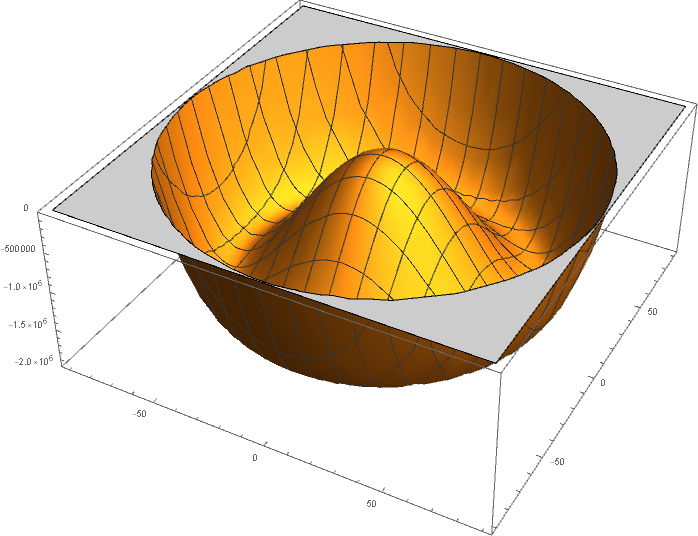
\includegraphics[width=10cm]{mexican_hat.png}
    \caption{Mexican hat potential with $\phi_1$,$\phi_2$ and $V(\phi_1,\phi_2)$ on the $x,y$ and $z$-axis}
    \label{fig:my_label1}
\end{figure}
The code used was:
\begin{lstlisting}
V[\[Phi]2_, \[Phi]1_] = -1/2*\[Mu]^2 (\[Phi]1^2 + \[Phi]2^2) + 
   1/4*\[Lambda] (\[Phi]1^2 + \[Phi]2^2)^2;
\[Mu] := 40;
\[Lambda] := 0.4;
Plot3D[V[\[Phi]2, \[Phi]1], {\[Phi]1, -90, 90}, {\[Phi]2, -90, 90}, 
 PlotRange -> {-2*10^6, 10^2}]
\end{lstlisting}
From the figure we easily see that even though there is an unstable saddlepoint at $V(\phi_1,\phi_2)=0$ this is not the minimum possible energy.

So the minimum energy is actually not at $V=0$ but at $V=$some negative value.

It is straightforward to see that this minimum value is in a circle of some radius $v^2=\phi_1^2+\phi_2^2$.

Inserting this into the potential and differentiating to find the minima we get:
\[
\partial_v V(v)=\partial_v \lp(\half \mu v^2+\frac{1}{4}\lambda v^4\rp)=0
\]
\[
\mu^2 v+\lambda v^3=0\Rightarrow v^2=-\frac{\mu^2}{\lambda}
\]
This new minima is called the "vacuum". If we want to expand around our minimum we then have to do it around this "true" minima and not 0.

Since we are expanding it is easier to look at the point where the complex part of the field is zero\footnote{We can do this since $\phi_1^2+\phi_2^2=v^2$ still can be satisfied, so this indeed is a minimum}. Now when we expand our Lagrangian around our minimum we are translated to the new position. 

Our field is then:
\[
\phi(x)=\frac{1}{\sqrt{2}}\lp(v+\eta(x)+i\xi(x) \rp)
\]
where $\eta(x)$ are the fluctuations in $\phi_1(x)$ and $\xi(x)$ in $\phi_2(x)$.

We've tried to illustrate the displaced position in figure \ref{fig:my_label2}
\begin{figure}[htb]
    \centering
    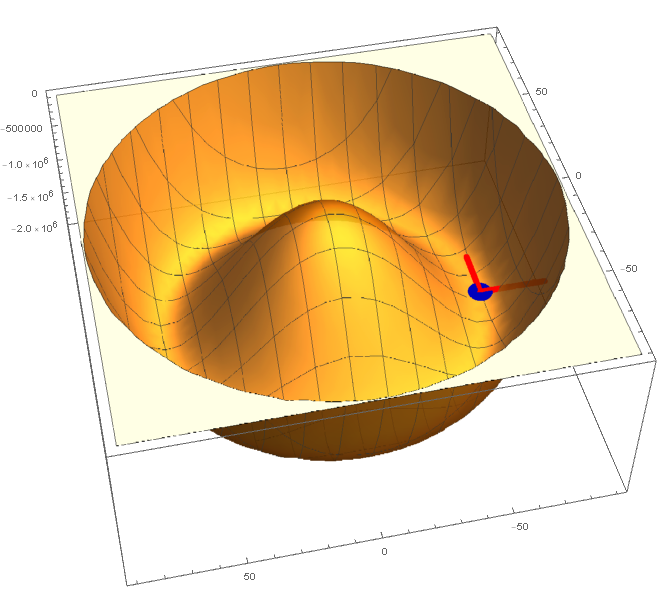
\includegraphics[width=10cm]{mexican_hat2.png}
    \caption{Mexican hat potential with $\phi_1$,$\phi_2$ and $V(\phi_1,\phi_2)$ on the $x,y$ and $z$-axis}
    \label{fig:my_label2}
\end{figure}
The code used was similar to the last:
\begin{lstlisting}
V[\[Phi]2_, \[Phi]1_] = -1/2*\[Mu]^2 (\[Phi]1^2 + \[Phi]2^2) + 
   1/4*\[Lambda] (\[Phi]1^2 + \[Phi]2^2)^2;
\[Mu] := 40;
\[Lambda] := 0.4;
P1 = Plot3D[{V[\[Phi]2, \[Phi]1]}, {\[Phi]1, -90, 90}, {\[Phi]2, -90, 
    90}, PlotRange -> {-2*10^6, 10^2}, PlotStyle -> Opacity[0.9], 
   Mesh -> Full];
P2 = Graphics3D[{Blue, Sphere[{0, -63, -1.5*10^6}, 5]}];
P3 = Graphics3D[{Red, Thickness[0.01], Arrowheads[Large], 
    Arrow[{{0, -63, -1.5*10^6}, {0, -90, -1.5*10^6}}]}];
P4 = Graphics3D[{Red, Thickness[0.01], Arrowheads[Large], 
    Arrow[{{0, -63, -1.5*10^6}, {20, -63, -1.5*10^6}}]}];
Show[P1, P2, P3, P4]
\end{lstlisting}
If we insert this into our original Lagrangian we get
\begin{align*}
\Lar'=&\frac{1}{2}\lp(\partial_\mu\lp(v+\eta(x)-i\xi(x)\rp)\rp)\lp(\partial^\mu\lp(v+\eta(x)+i\xi(x)\rp)\rp)\\
&-\mu^2\lp(v+\eta(x)-i\xi(x)\rp)\lp(v+\eta(x)+i\xi(x)\rp)-\lambda\lp(\lp(v+\eta(x)-i\xi(x)\rp)\lp(v+\eta(x)+i\xi(x)\rp) \rp)^2
\\
=&\half\partial_\mu\eta(x)\partial^\mu\eta(x)+\half\partial_\mu\xi(x)\partial^\mu\xi(x)\\
&\underbrace{+\frac{3}{2}\mu^2\eta^2-\half\mu^2\eta^2}_{\text{Interesting terms}}+\underbrace{\half\mu^2\xi^2-\half\mu^2\xi^2}_{\text{Interesting that cancels}}-\underbrace{\mu^2 v\eta-\half\mu^2v^2+\frac{1}{4}\mu^2v^2+\frac{1}{4}\frac{\mu^2\eta^4}{v^2}+\mu^2v\eta+\mu^2\eta^3+\frac{1}{4}\frac{\mu^2\xi^4}{v^2}+\frac{1}{2}\frac{\mu^2\eta^2\xi^2}{2v^2}+\mu^2\eta\xi^2}_{\text{Uninteresting terms}}\\
=&\half\partial_\mu\eta(x)\partial^\mu\eta(x)+\half\partial_\mu\xi(x)\partial^\mu\xi(x)+\mu^2\eta^2+\cdots
\end{align*}
We see that we end up with two traditional "kinetic" looking terms for the two fields since 
\[
\half\partial_\mu\eta(x)\partial^\mu\eta(x)\xrightarrow{\text{corresponds to}}\half \partial_\mu\phi\partial^\mu\phi
\]
and that we have a "mass-like" term for $\eta(x)$ since for our original Klein-Gordon Lagrangian
\be
\Lar=\half\partial_\mu\phi\partial^\mu\phi-\half m^2\phi^2
\ee
we got the equation of motion
\be
\lp(\Box^2-m^2\rp)\phi=0
\ee
where $m$ is the mass, so
\[
\mu^2\eta^2\xrightarrow{\text{corresponds to}}-\half m^2\phi^2
\]
This means that for our complex Lagrangian the $\eta$ mass is
\[
m_\eta=\sqrt{-2\mu^2}
\]
Now let us remember that the original Lagrangian was invariant under the global $U(1)$ transformation:
\[
\phi(x)\rightarrow \phi'(x)=e^{i\alpha}\phi(x)
\]
The translated field was
\[
\phi(x)\frac{1}{\sqrt{2}}\lp[ v+\eta(x)+i\xi(x) \rp]
\]
As opposed to the case without the translation, we now have terms where the $v$ shows up and all of the Sine and Cosine terms don't cancel. The $U(1)$-symmetry is then broken. This can be illustrated if we remember that $U(1)$ is isomorphic to $SO(2)$ in that a complex 1 dimensional function written in it's real and complex parts can be rotated in the complex plane by a $U(1)$ transformation.
\[
\begin{pmatrix}
\cos{\alpha}&-\sin{\alpha}\\
\sin{\theta }&\cos{\theta}
\end{pmatrix}
\begin{pmatrix}
\phi_1\\
\phi_2
\end{pmatrix}
=\begin{pmatrix}
\phi_1'\\
\phi_2'
\end{pmatrix}
\]
The rotation is shown in Figure \ref{fig:my_label3}.
\begin{figure}[htb]
    \centering
    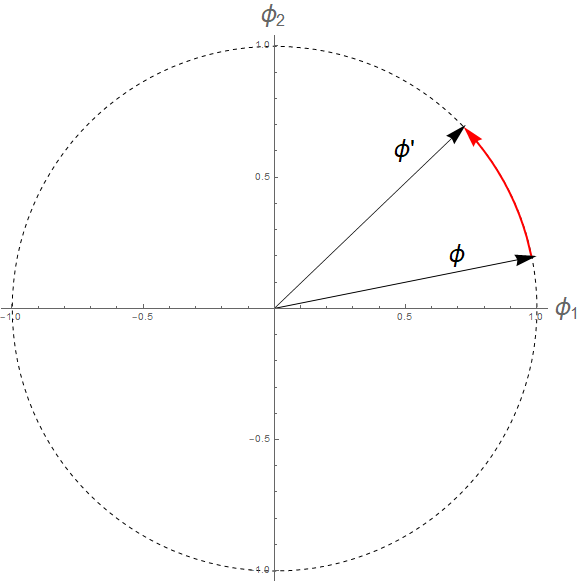
\includegraphics[width=8cm]{Rotation.png}
    \caption{Complex $U(1)$ rotation that corresponds to a $SO(2)$ rotation}
    \label{fig:my_label3}
\end{figure}

The code used was:
\begin{lstlisting}
P1 = Graphics[{Dashed, Circle[]}, Axes -> True, 
   AxesLabel -> {Style[Subscript[\[Phi], 1], Large], 
     Style[Subscript[\[Phi], 2], Large]}];
P2 = Graphics[{Red, Thick, 
    Arrow[BSplineCurve[
      Table[{Cos[x], Sin[x]}, {x, 0.2, Pi/4, Pi/100}]]]}];
P3 = Graphics[Arrow[{{0, 0}, {1, 0.2}}]];
P4 = Graphics[Arrow[{{0, 0}, {0.73, 0.7}}]];
P5 = Graphics[Text[Style["\[Phi]'", Large], {0.5, 0.6}]];
P6 = Graphics[Text[Style["\[Phi]", Large], {0.7, 0.2}]];
Show[P1, P2, P3, P4, P5, P6]
\end{lstlisting}
This lost mass terms known as a "Goldstone Boson". We see that we have a kinetic term so the particle must be there, but it has to be massless (or close to massless).

The lost mass can intuitively be seen from the plot of the potential where a particle can move freely along the the circle $v$ which is exactly in the $\xi$ direction. We can interpret this as the particle having small or no inertia.
\section{Chiral symmetries}
Let us take a look at the free QCD Lagrangian for quarks in flavour space $q=\begin{pmatrix}
    u\\
    d\\
    \vdots
\end{pmatrix}$:
\be
\Lar^0_{QCD}=-\frac{1}{4}G_{\mu\nu}^aG_a^{\mu\nu}+i\bar q_L\gamma^\mu D_\mu q_L+i\bar q_R\gamma^\mu D_\mu q_R
\ee
First let us note that the we have a left- and right-handed part and then a selfinteracting part which doesn't contain any quark parts. We'll use the common shorthand notation 
\[
\Lar^0_{QCD}="G^2"\:\:\:+\:\:\:"\bar q_L q_L"\:\:\:+\:\:\:"\bar q_R q_R"
\]
We will now examine a global flavour transformation of the left and righthanded quarks. The notation is 
\[
G\equiv SU(n_f)_L\ot SU(n_f)_R
\]
The flavourtransformations are
\begin{align}
q_L\xrightarrow{G}g_Lq_L,\:\:&\:\:q_R\xrightarrow{G}g_Rq_R\\
\bar q_L=q_L^\dagger \gamma^0\xrightarrow{G}\lp(g_L q_L\rp)^\dagger \gamma^0=q_L^\dagger g_L^\dagger \gamma^0,\:\:&\:\:\bar q_R=q_R^\dagger \gamma^0\xrightarrow{G}\lp(g_R q_R\rp)^\dagger \gamma^0=q_R^\dagger g_R^\dagger \gamma^0\\
\end{align}
where $g_{L,R}$ are elements of their individual $SU(n_f)_{L,R}$ groups. We let the transformation work and focus on the left part since the two others trivially follow. The transformed Lagrangian is:
\[
\Lar_{QCD}^0\xrightarrow{G}\Lar^{0'}_{QCD}="G^2"+iq_L^\dagger g_L^\dagger\gamma^0\gamma^\mu D_\mu g_L q_L+ "\bar q_R q_R"
\]
If we inspect the three middle terms, we see that since they don't have anything to do with the quarks flavours (they don't live in flavour space) they all commute with all the elements in $G$. Because of this, we can just let $g^{\dagger}$ act on $g$ getting the identity:
\[
\Lar_{QCD}^0\xrightarrow{G}\Lar^{0'}_{QCD}="G^2"+iq_L^\dagger \source{g_L^\dagger}\gamma^0\gamma^\mu D_\mu \target{g_L^{\phantom{l}}} q_L+ "\bar q_R q_R"=\Lar_{QCD}^0
\]
\drawarrows
So the Lagrangian is invariant under these flavourtranformations.
\section{Goldstone's theorem}

Here is a proof sketch for Goldstone's theorem. We have some Hamiltonian (or Lagrangian) with a continuous symmetry. This corresponds to a unitary operator which can be written as $e^{i\theta Q}$ where $Q$ is hermitian and $[H,Q]=0$. Let's choose our potential in a fashion such that our ground state solution (vacuum) has energy zero. This is just letting $H \rightarrow H+c$ and surely $H+c$ still has the same symmetry as $H$ since $c$ is a scalar and commute with everything. In short $H\ket{0}=0$. Now, the Hamiltonian has the symmetry but the solution, the state, might not. In spontaneous symmetry breaking the ground state will not be invariant under the symmetry transformation $Q\ket{0}\neq \ket{0}$. But since $H$ and $Q$ commute:

\be
0=[H,Q]\ket{0}=HQ\ket{0}-QH\ket{0}=H \lp( Q\ket{0} \rp)
\ee

So we have found another state with the same energy as the ground state. This state can be written as $Q\ket{0}=\int dx^3 J^{0}(\Bar{x},t) \ket{0}$ where $J^{0}(\Bar{x},t)$ is the conserved current. If we consider a state $\int dx^3 e^{-i\Bar{k}\cdot \Bar{x}}J^{0}(\Bar{x},t)\ket{0}$ we see(?) that this state has momentum $\hbar k$ and that it corresponds to the $Q\ket{0}$ state for zero momentum. Therefore the $Q\ket{0}$ state has energy and momentum zero and in relativistic theory this is just a massless particle.

The fact that we get one Goldstone boson for every broken symmetry generator assumes that two generators doens't give the same state $Q^a\ket{0}\neq Q^b\ket{0}$. Proof by contradiction: Assuming $Q^a\ket{0}= Q^b\ket{0}$ implies that $\mel{0}{[Q^a,Q^b]}{0}=0$ but $[Q^a,Q^b]=f_{abc}Q^c$ and $Q^c\ket{0}\neq \ket{0}$ so $\mel{0}{[Q^a,Q^b]}{0}=\mel{0}{f_{abc}Q^c}{0}\neq 0$.
\section{Explicit symmetry breaking}

The spontaneous symmetry breaking occurs only for the states and not for the underlying Lagrangian and only global symmetries can break spontaneously. Explicit symmetry breaking happens when terms in the lagrangian which break the symmetry are introduced. Let's see how a mass term can break the $\text{SU}(3)_L\ot\text{SU}(3)_R$ local symmetry of the QCD lagrangian. In the chiral basis:

\be 
q=
\begin{pmatrix}
    q_R\\
    q_L
\end{pmatrix} 
; \ 
\gamma_0=\begin{pmatrix}
    0&I\\
    I&0
\end{pmatrix}
; \ 
\gamma_5=\begin{pmatrix}
    I& 0\\
    0&-I
\end{pmatrix}
\ee

This basis makes the \textbf{algebra trivial} but of course the result is invariant of basis:
\be 
m\Bar{q}q = mq^\dag \gamma_0 q=m(q^{\dag}_{L}q_R+q^{\dag}_{R}q_{L})
\ee 

It is evident that this term breaks the combined $\text{SU}(3)_L\ot\text{SU}(3)_R$ but it retains a single $\text{SU}(3)_{R+L}$ symmetry. To see this, the idea is to rewrite the two independent left and right coupling group elements as a $\text{SU}(3)_{R+L}$ group element and a $\text{SU}(3)_{R-L}$ group element:

\be
g_R=e^{i\theta^{a}_R \lambda^a}; \ g_L=e^{i\theta^{a}_L \lambda^a} \ \rightarrow \ g_{R+L}=e^{i\theta^{a} \lambda^a}; \ g_{R-L}=e^{i\gamma_5\theta^{a}_5 \lambda^a}
\ee 

So $g_R$ and $g_L$ rotate the right handed and left handed independently whereas $g_{R+L}$ rotates them both by the same amount in the same direction and lastly $g_{R-L}$ rotates right handed and left handed states by the same amount but in opposite directions. This is due to the fact that $q_{R/L}$ are eigenstates of $\gamma_5$ with eigenvalues $\pm1$, but let's see this explicitly:

\be
g_{R-L}q=e^{i\theta^{a}_5\lambda^a}e^{\gamma_5} \begin{pmatrix}
    q_R\\
    q_L
\end{pmatrix} = e^{i\theta^{a}_5\lambda^a}(1+\gamma_5+\half I+...) \begin{pmatrix}
    q_R\\
    q_L
\end{pmatrix} = e^{i\theta^{a}_5\lambda^a}\begin{pmatrix}
    e\cdot q_R\\
    e^{-1}\cdot q_L
\end{pmatrix}
\ee

In the first equality the Baker-Campbell-Hausdorff formula is applied and in the second I use $\gamma_5^2=I$. The two formulations of the groups are equivalent and in the latter picture it is clear that only the $\text{SU}(3)_{R-L}$ symmetry is broken. So in the end, even though both $\text{SU}(3)_L\ot\text{SU}(3)_R$ symmetries are broken a combined $\text{SU}(3)_{R+L}$ symmetry rises from the ashes.

\section{Identifying terms in global ChPT Lagrangian}
We've just seen how a mass term can break the Chiral symmetry of the Lagrangian explicitly.

Now let's embark on a "gedankenexperiment". If we imagine that the mass term (now $m$ is a hermitian matrix in flavor space) transforms globally as:
\be
m\rightarrow g_L m g_R^\dagger
\ee
the mass term won't break the symmetry of the Lagrangian. In fact we can now create multiple terms that keep this symmetry. We want this because this terms can add up to create an "effective Lagrangian" which breaks the symmetry in the same way that the QCD Lagrangian does.

We have to note that since we want the Lagrangian to be a number and our operators now are matrices, we have to take the trace of everything we do. The notation for this will (confusingly) be $\Tr[A]=\expval{A}$.

We will work with the Goldstone field $U$, which transforms as
\begin{align}
    U&\rightarrow g_R U g_L^\dagger\\
    U^\dagger&\rightarrow g_L U^\dagger g_R^\dagger
\end{align}

The first terms in the Lagrangian could be
\[
\Lar=\expval{UU^\dagger}=\expval{I}=\dim{U}
\]
but this is trivial and is generally not regarded as a term, since when inserting into the Euler-Lagrange equation it will vanish anyway.

Now if we start using derivatives a plethora of options opens up. The derivative transforms as:
\begin{align}
\partial_\mu U & \rightarrow g_R\partial_\mu Ug_L^\dagger\\
\partial_\mu U^\dagger & \rightarrow g_L\partial_\mu U^\dagger g_R^\dagger
\end{align}
Let's now set up terms which include $m$ or $U$ or both:
\begin{align*}
    \Lar_{\text{eff}}=&C_1\expval{\partial_\mu U \partial^\mu U^\dagger}+C_2\expval{mU+(Um)^\dagger}+C_3\expval{mU-(Um)^\dagger}+C_4\expval{m\partial_\mu U+\lp(\partial^\mu U m\rp)^\dagger}\\
    & C_5\expval{\partial_\mu U^\dagger\partial_\nu U}\expval{\partial^\mu U^\dagger\partial^\nu U}+C_6\expval{m^\dagger m}+\cdots
\end{align*}
Note that the $C_4$-term is not allowed since it is not Lorentz invariant nor a scalar. We'll quickly just show that a couple of the terms satisfies the invariance:
\[
C_2\expval{mU+m^\dagger U^\dagger}\rightarrow C_2\expval{g_Lm\underbrace{g_R^\dagger g_R}_{I}U g_L^\dagger+g_Rm\underbrace{g_L^\dagger g_L }_{I}U^\dagger g_R^\dagger}=C_2\expval{g_LmU g_L^\dagger+g_Rm U^\dagger g_R^\dagger}
\]
Using the cyclic and distributive properties of the trace\footnote{$\expval{AB}=\expval{BA}$ and $\expval{A+B}=\expval{A}+\expval{B}$} we just get:
\[
C_2\expval{g_L^\dagger g_LmU+g_R^\dagger g_Rm U^\dagger}=C_2\expval{mU+m^\dagger U^\dagger}
\]
So the term is invariant.
\section{What \underline{\textit{is}} a field theory?}

We recall our very first introduction to classical field theory, the string:

\be
\Lar = \mathscr{T}-\mathscr{V} = \half\sigma \lp(\pdv{u}{t}\rp)^2-\half\tau\lp(\pdv{u}{x}\rp)^2
\ee

Where $\sigma$ is the mass density, $\tau$ is the string tension and $u$ is the displacement from the equilibrium position. We see that kinetic energy arises through a time dependent change in the displacement at a specific point. This can happen when a moving wave glides past the point of interest and this is generally how a kinetic term is introduced. The potential energy, however, is associated with the slope of the string and is something specific to our example and will change depending on the system in question. 

In quantum field theory the Lagrangian, and especially the potential, is not something that is specific to the system considered, rather, it is general because it explains how nature \textbf{\textit{is}}. The QCD Lagrangian is the QCD Lagrangian regardless of what aspect you're trying to study and therefore the Lagrangian should be regarded as something inherent to nature. 

Let's now take a look at what the field is, through the familiar $\phi^4$-Lagrangian:

\be
\Lar=\lp(\partial_\mu\phi\rp)^*\lp(\partial^\mu\phi\rp)-\mu^2\phi^*\phi-\lambda\lp(\phi^*\phi \rp)^2
\ee

The postulate is that this Lagrangian explains some inherent aspect of nature, in this case mass acquisition. The field is then what we solve for in the equation when the Euler-Lagrange equation is applied and should therefore account for what the particles actually do. The field can be interpreted as 'all' the possible wave functions combined in one entity. The Euler-Lagrange equation we arrive at is probably not one we can straightforwardly solve and is probably not even analytically solvable either. Therefore we must look for some pertubative solution and it is natural to do this around local minima. In this case, and in most(!), the potential around the minima will look like the familiar harmonic oscillator potential. This gives rise to solutions with energies linear in the relevant quantum number. Now we will interpret the physical particles as excitations to this field and the states are then the actual solutions to the Euler-Lagrange equation. Here are some highlights of the above discussion: 
\begin{itemize}
    \item The QFT Lagrangian describes nature, that is, it is some underlying feature of nature that tells how particles (fields) are.
    \item The field is in some sense all possible wave functions we can have and can therefore account for both 1 particle and 100 particles. 
    \item The particles are the excitations to the field.
    \item A state is a (pertubative) solution to the Euler-Lagrange equation and is indexed by an associated quantum number.
\end{itemize}
\section{Path Integrals}
\subsection{Background}
In Quantum Mechanics we are used to seeing the Schrödinger equation
\be
i\hbar \partial_t\ket{\Psi}=\ham \ket{\Psi}
\ee
where the capital $\Psi$'s imply a timedependent state. 

The equation is easily solveable and gives the standard exponential solution
\be
\ket{\Psi}=e^{-\frac{i}{\hbar}\ham t}\ket{\psi}
\ee
where the $\ket{\psi}$ is the initial state of the system. The exponential terms is commonly referred to as the "propagator" since it propagates the state in time. This is written as:
\be
\ket{\Psi}=U(x,t)\ket{\psi} 
\ee
If we already know the initial state the task then seems trivial - just calculate the propagator and you will know how the state behaves at any point in time. The usual way to do this is by solving the eigenvalue equation:
\be \label{eq:propagator}
\ham\ket{n}=E_n\ket{n}
\ee
rendering the propagator
\be
U(x,t)=\sum_n\ket{n}\bra{n}e^{-\frac{i}{\hbar}E_nt}
\ee

We will now present a different way to directly calculate the propagator given in equation \ref{eq:propagator}. As opposed to the Schrödinger approach, which builds on the Hamiltonian formalism we will now instead use the Lagrangian and the principle of least action.
\subsection{Conceptually}
First let us imagine a particle going from one point (a) to another (b) between time $t_a$ and $t_b$. This is illustrated in figure \ref{fig:my_label4}.
\begin{figure}[htb]
    \centering
    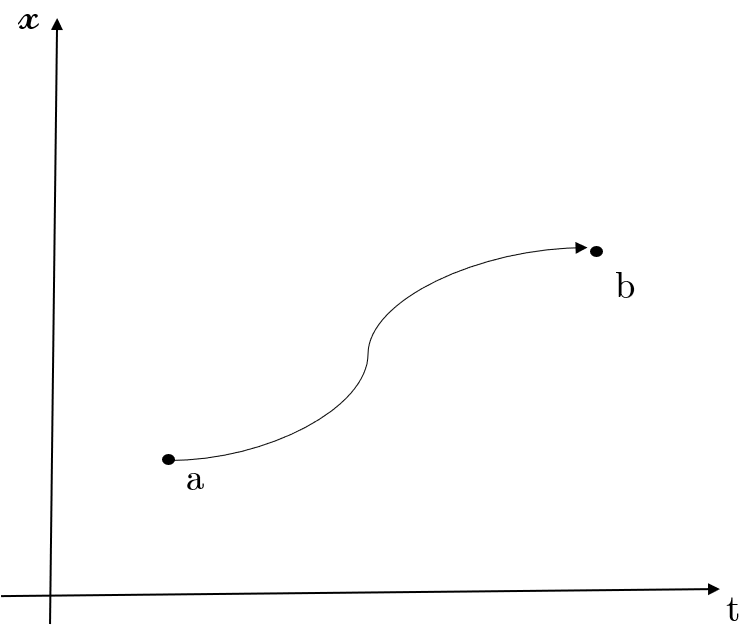
\includegraphics[width=8cm]{Pathint.PNG}
    \caption{Caption}
    \label{fig:my_label4}
\end{figure}

The question is now: \textit{which path does the particle take}?

Classicly we would expect the particle to want to "minimize the action integral":
\be
S=\int_{t_a}^{t_b} \mathcal{L}(x,\dot{x},t)\:\dd t
\ee
But what about all the other possible paths?

Well, according to quantum mechanics does the particle not only have the possibility of taking every other path, it actually does so - at once!

So not only do we have to account for the classical path taken - we have to account for every possible path. This seems like an impossible task but we'll give it a try,
\begin{figure}[htb]
    \centering
    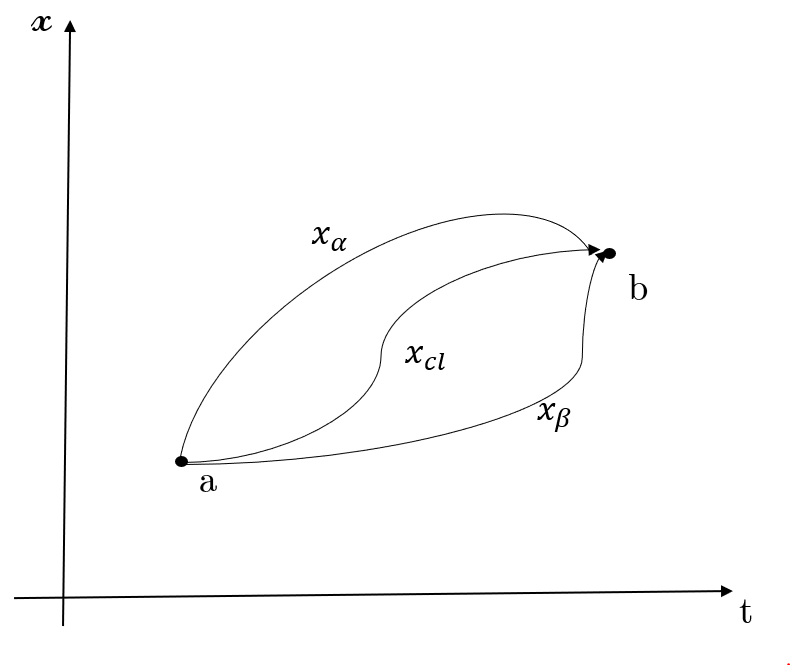
\includegraphics[width=9cm]{Pathint2.PNG}
    \caption{Caption}
    \label{fig:my_label5}
\end{figure}

Now "what does all of this have to do with the propagator?" one might ask. It turns out that a different formulation not involving the Hamiltonian, but instead the action is
\[
U(x,t;x',t')=A\sum_{\text{all paths}}e^{\frac{i}{\hbar} S[x(t)]}
\]
where $A$ is some normalization constant. Pretty easy right? All we have to do is take and infinite amount of paths, integrate over them and then sum over an infinite amount of exponential involving these integrals.

Obviously this isn't as easy as we though, but let's go ahead and do it for few specific cases and maybe we'll learn some tricks along the way.
\subsection{A few examples}
\subsubsection{The free particle exact}
The notation used in path integrals is:
\be
U(x_N,t_N;x_0,t_0)=A\int^{t_N}_{t_0}e^{\frac{i}{\hbar}S[x(t)]}\PD[x(t)]
\ee
where the script "\textit{D}" implies that you have to integrate over every path. 

The way to do this is by discretizing every path in the way shown in Figure \ref{fig:my_label6}.

\begin{figure}[htb]
    \centering
    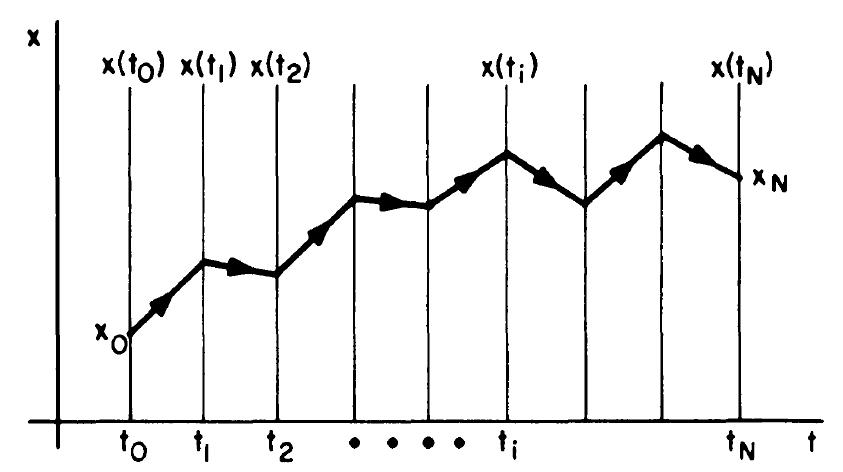
\includegraphics[width=8cm]{discrete.PNG}
    \caption{Caption}
    \label{fig:my_label6}
\end{figure}

So for the free particle we want to replace the action integral with a discrete sum:
\be
S[x(t)]=\half m\int_{x_0}^{x_N}\dot{x}^2 \:\dd t\rightarrow\lim_{\substack{N\rightarrow\infty\\\epsilon\:\rightarrow\:0}} \half m \sum_{i=0}^{N-1}\frac{\lp(x_{i+1}-x_i\rp)^2}{\epsilon}
\ee
Let us plug this into the equation for the propagator:
\[
U(x_N,t_N;x_0,t_0)=A\lim_{\substack{N\rightarrow\infty\\\epsilon\:\rightarrow\:0}} \int_{-\infty}^{\infty}\int_{-\infty}^{\infty}\cdots\int_{-\infty}^{\infty}e^{\frac{i}{\hbar}\half m \sum_{i=0}^{N-1}\lp(\frac{x_{i+1}-x_i}{\epsilon}\rp)^2}\:\dd x_1\:\dd x_2\cdots\dd x_{N-1}
\]
We can make this a little easier to look at by defining
\[
\alpha\equiv-\frac{im}{2\hbar\epsilon}
\]
leaving us with:
\[
U(x_N,t_N;x_0,t_0)=A\lim_{\substack{N\rightarrow\infty\\\epsilon\:\rightarrow\:0}} \int_{-\infty}^{\infty}\int_{-\infty}^{\infty}\cdots\int_{-\infty}^{\infty}e^{\alpha \sum_{i=0}^{N-1}\lp(x_{i+1}-x_i\rp)^2}\:\dd x_1\:\dd x_2\cdots\dd x_{N-1}
\]
Let us first do the integral over $x_1$ and let us call that $U_1$:
\[
U_1=\int_{-\infty}^{\infty}e^{-\alpha\lp[\lp(x_1-x_0\rp)^2+\lp(x_2-x_1\rp)^2\rp]}\:\dd x_1
\]
This just corresponds to a displaced gaussian integral with solution
\[
U_1=\lp(\frac{\pi}{2\alpha}\rp)^\half e^{-\half\alpha\lp[x_2-x_0\rp]^2}
\]
Proceeding to $U_2$ we then have a new integral:
\[
U_2=\lp(\frac{\pi}{2\alpha}\rp)^\half\int_{-\infty}^{\infty}e^{-\alpha\lp[\lp(x_3-x_2\rp)^2+\frac{1}{2}\lp(x_2-x_0\rp)^2\rp]}\:\dd x_2=\lp(\frac{\pi^2}{3\alpha^2}\rp)^\half e^{-\frac{1}{3}\alpha[x_3-x_0]^2}
\]
We see that after the $N-1$ itterations we would get
\[
U(x_N,t_N;x_0,t_0)=A\frac{\pi^{\frac{(N-1)}{2}}}{N^{\half}\alpha^{\frac{N-1}{2}}}e^{-\frac{\alpha}{N}\lp[x_N-x_0\rp]^2}
\]
Putting our $\alpha$ back in and grouping terms of equal power we get:
\[
U(x_N,t_N;x_0,t_0)=A\lp(\frac{2\pi\hbar\epsilon i}{m}\rp)^{\frac{N}{2}}\lp(\frac{m}{2\pi \hbar i N\epsilon}\rp)^{\frac{1}{2}}e^{\frac{im\lp[x_N-x_0\rp]^2}{2\hbar N\epsilon}}
\]
Since $\epsilon$ was the time stepsize, it must follow that $N\epsilon=\Delta t=t_N-t_0$. We also see that if we set $A$ to be the inverse of the fist term we are left with the correct propagator
\be
U(x_N,t_N;x_0,t_0)=\lp(\frac{m}{2\pi \hbar i \Delta t}\rp)^{\frac{1}{2}}e^{\frac{im[\Delta x]^2}{2\hbar \Delta t}}\hspace*{1cm}\checkmark
\ee
\subsubsection{Using the classical action}
Okay so now we have gone through the tedious procedure of calculating the exact propagator. 
\section{The Gell-Mann-Oakes-Renner mass relation}
We have seen how to construct an effective Lagrangian with terms that break Chiral symmetry in the same way as in the original QCD Lagrangian. 

We will now show how to use this Lagrangian to determine a relation between the quark and pion masses.

To second order our effective Lagrangian was (we can use $\partial_\mu$ and $D_\mu$ interchangeably since we only care for the coefficient in front and if we write $D_\mu$ in the effective Lagrangian we would also write it in the Klein-Gordon Lagrangian) : 

\be
\Lar_{\text{eff}}^{(2)}=\frac{f^2}{4}\expval{\partial_\mu U^\dagger \partial^\mu U+U^\dagger\chi+\chi^\dagger U}
\ee
where $\chi$ is the mass term given by:
\be
\chi=2B_0\lp(x+ip\rp)
\ee

Just as in the case with the Klein Gordon Lagrangian we have to choose a direction in complex space for us to break chiral symmetry. We choose:
\be
p=0,\:\:\:s=\mathcal{M}=
\begin{pmatrix}
m_u & 0 & 0\\
0 & m_d & 0\\
0 & 0 & m_s\\
\end{pmatrix}
\ee

Since $\mathcal{M}$ is now hermitian and using cyclic permutation under trace we can just write the effective Lagrangian as
\be \label{eq:GSLar}
\Lar_{\text{eff}}^{(2)}=\frac{f^2}{4}\expval{\partial_\mu U^\dagger \partial^\mu U +2B_0\mathcal{M}\lp( U^\dagger+U \rp)}
\ee
where we have used the cyclic proporties of the trace to get $\mathcal{M}$ on the left of both $U$ and $U^\dagger$

Since the Goldstone fields live in the coset space $\text{SU}(3)_{R-L}=(\text{SU}(3)_R\ot \text{SU}(3)_L)/\text{SU}(3)_{R+L}$ it is natural to write $U$ as a special unitary matrix:
\be
U(\Phi)=\exp[i\frac{\sqrt{2}}{f}\Phi]
\ee
where $\Phi$ is the Hermitian matrix
\be
\Phi=\begin{pmatrix}
    \frac{1}{\sqrt{2}}\pi^0+\frac{1}{\sqrt{6}}\eta_8 & \pi^+ & K^+\\
    \pi^-& -\frac{1}{\sqrt{2}}\pi^0+\frac{1}{\sqrt{6}}\eta_8& K^0\\
    K^-&\bar{K}^0 &-\frac{2}{\sqrt{6}}\eta_8
\end{pmatrix}
\ee
For our purpose we are only interested in the Pion fields, so we can write it as
\be
\Phi\simeq\begin{pmatrix}
    0 & \pi^+ & 0\\
    \pi^-& 0 & 0\\
    0 & 0 & 0
\end{pmatrix}
\ee
And the square of the matrix is (we'll use this later)
\be
\Phi^2\simeq\begin{pmatrix}
    \pi^+\pi^- & 0 & 0\\
    0 & \pi^+\pi^- & 0\\
    0 & 0 & 0
\end{pmatrix}
\ee
We will now expand the Goldstone field in terms of the matrix $\Psi$. We want everything in the Lagrangian to be of order $\sim \Phi^2$ so for the matrix it self we get:
\begin{align*}
U(\Phi)&\simeq I+i\frac{\sqrt{2}}{f}\Phi-\frac{1}{f^2}\Phi^2+\mathcal{O}(\Phi^3)\\
U^\dagger(\Phi)&\simeq I-i\frac{\sqrt{2}}{f}\Phi-\frac{1}{f^2}\Phi^2+\mathcal{O}(\Phi^3)
\end{align*}
For the derivative since we multiply the two together we only need to expand the matrix to first order:
\begin{align*}
\partial^\mu U(\Phi)&\simeq i\frac{\sqrt{2}}{f}\partial^\mu\Phi+\mathcal{O}(\Phi^2)\\
\partial_\mu U^\dagger(\Phi)&\simeq -i\frac{\sqrt{2}}{f}\partial_\mu\Phi+\mathcal{O}(\Phi^2)\\
\end{align*}
The mass term of the Lagrangian (eq: \ref{eq:GSLar}) then becomes:
\[
\mathcal{M}\lp[U^\dagger(\Phi)+U(\Phi) \rp]\simeq \mathcal{M}\lp[ I+I+i\frac{\sqrt{2}}{f}\Phi-i\frac{\sqrt{2}}{f}\Phi-\frac{1}{f^2}\Phi^2-\frac{1}{f^2}\Phi^2+\mathcal{O}(\Phi^3) \rp]=-\frac{2}{f^2}\mathcal{M} \Phi^2
\]
while the kinetic term is
\[
\partial^\mu U(\Phi)\partial_\mu U^\dagger(\Phi)\simeq\frac{2}{f^2}\partial_\mu\Phi\partial^\mu\Phi
\]
Leaving us with the simplified:
\be
\Lar_{ \text{eff}}^{(2)}\simeq\expval{ \half\partial_\mu\Phi\partial^\mu\Phi-B_0\mathcal{M}\Phi^2}
\ee
Let us now calculate the actual trace of the matrices:
\begin{align*}
    \Lar_{ \text{eff}}^{(2)}&\simeq
\expval{
\half
\begin{pmatrix}
0 &\partial_\mu \pi^+& 0\\
\partial_\mu \pi^- &0 & 0\\
0 & 0 & 0
\end{pmatrix}
\begin{pmatrix}
0 &\partial^\mu \pi^+& 0\\
\partial^\mu \pi^- &0 & 0\\
0 & 0 & 0
\end{pmatrix}
-B_0
\begin{pmatrix}
m_u & 0 & 0\\
0 & m_d & 0\\
0 & 0 & m_s\\
\end{pmatrix}
\begin{pmatrix}
    \pi^+\pi^- & 0 & 0\\
    0 & \pi^+\pi^- & 0\\
    0 & 0 & 0
\end{pmatrix}
}\\
&=
\expval{
\half
\begin{pmatrix}
\partial_\mu \pi^+ \partial^\mu \pi^- & 0 & 0\\
0 & \partial_\mu \pi^- \partial^\mu \pi^+ & 0\\
0 & 0 & 0
\end{pmatrix}
-B_0
\begin{pmatrix}
    m_u\pi^+\pi^- & 0 & 0\\
    0 & m_d\pi^+\pi^- & 0\\
    0 & 0 & 0
\end{pmatrix}
}\\
&=\half\lp[\partial_\mu \pi^+ \partial^\mu \pi^-+ \partial_\mu \pi^- \partial^\mu \pi^+ \rp]-B_0\lp[ m_u\pi^+\pi^-+ m_d\pi^+\pi^- \rp] 
\end{align*}
For the kinetic term we can switch the lower and upper indices since we are summing over them anyway and our final Lagrangian is:
\be \label{eq:finLar}
\Lar_{\text{eff}}^{(2)}\simeq \partial_\mu \pi^+\partial^\mu \pi^- -B_0\lp[m_u+m_d \rp]\pi^-\pi^+
\ee
If we remind our self that the the two pion fields are each others complex conjugate ($\Phi$ is hermitian):
\[
\lp(\pi^+ \rp)^*=\pi^-
\]
and then check equation \ref{eq:finLar} up against the original complex Klein-Gordon Lagrangian
\be
\Lar_{KG}=\lp(\partial_\mu \phi\rp)^* \lp(\partial^\mu \phi\rp) - m^2\phi^*\phi
\ee
We remember that the prefactor in front of the $\phi^*\phi$ gave rise to a mass term when inserted into the Euler Lagrangian equation. Another important thing to remember is that the factor in front of the kinetic term has to correspond to the factor in front of the mass term. In this case this factor is just 1 and all of this leads us to conclude that
\be
M_{\pi^\pm}^2=B_0\lp[m_u+m_d \rp]
\ee
In the limit where the quark masses are equal to each other $m_u=m_d=m_q$ (which they almost are) we just get:
\be
M_{\pi^\pm}^2=2B_0 m_q
\ee

\section{Counting-schemes in ChPT}
The QCD partition function at low temperatures can be calculated using effective ChPT:
\[
Z=\expval{e^{-\beta \ham}}=\int \exp[-\int_{V_4}\:\dd x \Lar]\:\PD[U]
\]
where $\Tr[A]=\expval{A}$, $\PD[U]$ marks a path integral over the pion field $U(x)$ living in $SU(n_f)$ on the surface of a four-dimensional torus of volume $V=L\times L\times L\times \beta$ \edit{(Svend: We need further comments on this as we understand it)}.

We have shown that that an infinite amount of terms can be written for the effective Lagrangian. We have to find a way to a way to determine which terms we will actually use. 

The first counting scheme is the \textit{p-counting} or momentum counting scheme. The differential operator $\partial_\mu$ is of course the momentum and then is of order $p$. The typical length scale of a meson (pion for example) is it's wavelength which is inversely proportional to its momentum so $p\sim\frac{1}{L}$. What about the masses of the pion and quarks? Here we get the freedom to choose the order of the masses and that separates $p$- and $\epsilon$-counting. First of all we remember that $m_q\sim m_\pi^2$ from the Gell-Mann-Oakes-Renner mass relation.  In $p$-counting it is natural to take $m_\pi\sim p$ due to the mass-momentum relation. It is important to note that taking the pion mass to zero is equivalent to taking the box size (of characteristic length $L$) to infinity. However in $\epsilon$-counting we consider the case where the box may remain finite when the pion mass approaching zero. That is $m_\pi \ll L$ such that $m_\pi \sim \epsilon^2$. This is a different regime and it will prove very interesting (Gasser-Leutwyler). An overview of the different counting schemes are presented in table \ref{tab:my_label1}.

\edit{Svend: Jeg har lavet en respons til nedenstående da der mangler noget. Jeg ved ikke om nedenstående er overflødigt nu eller om det skal tilføjes ovenstående.}
Let us first define the whole universe as our playing ground. If assume a large but finite size we can define a large length scale $L$,a small temperature $T$. Since we are looking at Pion fields it also makes sense to look at these on the scale of \edit{(more on differences between p and $\epsilon$ counting)} These are our control parameters and their different weights in the different counting schemes are shown in table \ref{tab:my_label1}.
\begin{table}[htb]
    \centering
    \begin{tabular}{c|c|c}
        Term & $p$-counting & $\epsilon$-counting\\
        \hline\hline
        $\partial_\mu$ & $\BigO(p)$  & $\BigO(\epsilon)$\\
        \hline
        $m_q$ & $\BigO(p^2)$ & $\BigO(\epsilon^4)$\\
        \hline
        $M_{\pi^\pm}$ & $\BigO(p)$ & $\BigO(\epsilon^2)$ \\
        \hline
        $\frac{1}{L}$ & $\BigO(p)$ & $\BigO(\epsilon)$ \\
        \hline
        $T$ & $\BigO(p)$ & $\BigO(\epsilon)$ 
    \end{tabular}
    \caption{Counting schemes in ChPT}
    \label{tab:my_label1}
\end{table}

To lowest order (2) the effective Lagrangian is the one used to show the Gell-Mann-Oakes-Renner mass relation:
\[
\Lar_{\text{eff}}^{(2)}=\frac{f^2}{4}\expval{\partial_\mu U^\dagger \partial^\mu U +2B_0\mathcal{M}\lp( U^\dagger+U \rp)}
\]

This is the one we will be treating.
\subsection{$\epsilon$-counting}
We will proceed to now use the $\epsilon$-counting scheme. Rather than expanding U around 1 we now choose an arbitrary direction $u^2=U_0$ \edit{(er det ikke $e^{i\xi}$ som står for at vælge retning?)}. The Goldstone field is then
\be
U(x)=ue^{i\xi(x)}u,\:\:\:u\in SU(n_f)\:\:\:\text{and}\:\:\:\xi(x)=\sum_{n\neq 0}q_n^a\lambda_au_n(x)
\ee
First we expand our field to second order:
\begin{align*}
U(\xi)&\simeq U_0\lp[ I+i\xi-\frac{1}{2}\xi^2+\mathcal{O}(\xi^3)\rp]\\
U^\dagger(\xi)&\simeq U_0^\dagger\lp[ I-i\xi-\frac{1}{2}\xi^2+\mathcal{O}(\xi^3)\rp]
\end{align*}

\begin{align*}
\partial^\mu U(\xi)&\simeq iU_0\partial^\mu\xi+\mathcal{O}(\xi^2)\\
\partial_\mu U^\dagger(\xi)&\simeq -iU_0^\dagger \partial_\mu\xi+\mathcal{O}(\xi^2)\\
\end{align*}
The mass term of the Lagrangian (eq: \ref{eq:GSLar}) then becomes:
\[
2B_0\mathcal{M}\lp[U^\dagger(\xi)+U(\xi) \rp]\simeq 2B_0\mathcal{M}\lp[ U_0+U_0^\dagger+iU_0\xi-iU_0^\dagger\xi-\frac{1}{2}U_0\xi^2-\frac{1}{2} U_0^\dagger \xi^2+\mathcal{O}(\xi^3) \rp]
\]
\[
=2B_0\mathcal{M}\lp[U_0^\dagger+U_0 \rp]+2i\xi B_0\mathcal{M}\lp[U_0^\dagger-U_0 \rp]-\frac{1}{2} B_0\mathcal{M}\xi^2\lp[U_0^\dagger+U_0 \rp]
\]
while the kinetic term is
\[
\partial^\mu U(\xi)\partial_\mu U^\dagger(\xi)\simeq \partial_\mu\xi\partial^\mu\xi
\]
Inserting this into the Lagrangian gives:
\[
\LeadLar =\frac{f^2}{4}\expval{\partial_\mu\xi\partial^\mu\xi+2B_0\mathcal{M}\lp[U_0^\dagger+U_0 \rp]+2i\xi B_0\mathcal{M}\lp[U_0^\dagger-U_0 \rp]-\frac{1}{2} B_0\mathcal{M}\xi^2\lp[U_0^\dagger+U_0 \rp]}
\]
Inserting this into the partition function:
\[
Z=\int\exp[\int\frac{f^2}{4}\expval{\partial_\mu\xi\partial^\mu\xi+2B_0\mathcal{M}\lp[U_0^\dagger+U_0 \rp]+2i\xi B_0\mathcal{M}\lp[U_0^\dagger-U_0 \rp]-\frac{1}{2} B_0\mathcal{M}\xi^2\lp[U_0^\dagger+U_0 \rp]}\:\dd x ]\:\PD[U]
\]
We now have to determine of what order the different terms contribute to this exponential. We want a kinetic term in our final Lagrangian so it makes sense to start of by giving this the appropriate weight. 

We know that the product of the two derivatives give us something of order $\BigO(\epsilon^2)$. We also know that when integrating over the volume \edit{(of the 4-torus $L\times L\times L\times \beta$??)} we'll get a contribution of order $\BigO(\epsilon^{-4})$. 

So for the kinetic term to be of order 1 the field most be of order $\xi(x)\sim \BigO(\epsilon)$. We can now use this and the counting scheme established in table \ref{tab:my_label1} to identify the order of all the terms in our partitionfunction:
\[
Z=\int\exp[\int\frac{f^2}{4}\expval{\underbrace{\partial_\mu\xi\partial^\mu\xi}_{\mathcal{O}(\epsilon^4)}+\underbrace{2B_0\mathcal{M}\lp[U_0^\dagger+U_0 \rp]}_{\text{constant of order }\mathcal{O}(\epsilon^4) }+\underbrace{2i\xi B_0\mathcal{M}\lp[U_0^\dagger-U_0 \rp]}_{\BigO(\epsilon^5)}-\underbrace{\frac{1}{2} B_0\mathcal{M}\xi^2\lp[U_0^\dagger+U_0 \rp]}_{\text{mass term of order }\BigO(\epsilon^6)}}\:\dd x ]\:\PD[U]
\]
Like we just wrote, integrating over the volume will give us contribution on the order of $V\sim \BigO (\epsilon^{-4})$. This means that all terms of higher order than $\epsilon^4$ can be thrown away:
\[
Z=\int\exp[\frac{f^2B_0Vm_q}{2}\Re\expval{U_0 }+\int\frac{f^2}{4}\expval{\partial_\mu\xi\partial^\mu\xi}\:\dd x ]\:\PD[U]
\]
Where we for the first term have used that $\expval{U_0^\dagger+U_0}=2\Re\expval{U_0}$, and we have assumed that $m_u=m_d=m_q$.

It's seems reasonable to assume that we can factor the integral. \edit{This can be shown explicitly}. For now let us just do it:
\be
Z=F(\xi)\times\int_{SU(N)} e^{s\Re\expval{U_0}}\:\dd\mu( U),\hspace*{1.5cm}s\equiv \frac{f^2B_0Vm_q}{2}
\ee
Where $F(\xi)$ is the path integral part of the partition function and the integral is over the group $SU(N)$.

If we want to calculate QCD features using this partition function, we have to compute it's generating functional. This is given by
\[
\partial_{m_q} \log Z = \frac{1}{Z}\partial_{m_q} Z
\]
We are differentiating w.r.t the mass term. For the quarks this mass term shows up in the Hamiltonian as $m_q \bar q q$. So for the term $\partial_\mu Z$ we just get a factor $\bar q q$ out of the exponential (this can also be seen explicitly):
\[
\frac{1}{Z}\partial_{m_q} Z=\frac{1}{Z}\expval{\bar q q e^{-\beta \ham}}=\mel{0}{\bar q q}{0}
\]
which is just the quark-condensate. Note that the quark condensate is extensive in the volume $V$.

We see that the we won't even need the path integral part since it doesn't depend on $m_q$ and we only have to calculate the group integral. For simplicity we can start out with only calculating over $U(1)$.

Here all the values in the group can be reached by
\[
U_0=e^{i\theta}
\]
with $\theta$ going from 0 to $2\pi$. The appropriate (Haar) measure \edit{(we would like to understand this better?)} is then $d\theta$ which is easily normalized:
\be
1=A\int_{0}^{2\pi}d\theta=A2\pi \Longleftrightarrow A=\frac{1}{2\pi}
\ee

So the normalized measure is $\frac{d\theta}{2\pi}$. For U$(1)$ the group integral looks like:
\be
\int_{0}^{2\pi} \frac{1}{2\pi} e^{s\Re{e^{i\theta}}}  d\theta = \int_{0}^{\pi} \frac{1}{\pi} e^{s\cos(\theta)} d\theta
\ee

Where we have used that $\cos(\theta)$ is an even function. The calculations continue with expressing the exponential as its Maclaurin series and commuting the integral and sum \edit{(when is this okay? - Fubini/Tonelli)}:

\be
 \frac{1}{\pi}\int_{0}^{\pi}\sum_{n=0}^{\infty}\frac{s^n\cos^n(\theta)}{n!}d\theta = \frac{1}{\pi}\sum_{n=0}^{\infty}\int_{0}^{\pi}\frac{s^n\cos^n(\theta)}{n!}d\theta
\ee

But $\cos^{2m+1}(\theta)$ is odd and integrates to zero and for even $n$ the integral can be looked up: 

\be
\frac{1}{\pi}\sum_{m=0}^{\infty}\int_{0}^{\pi}\frac{s^{2m}\cos^{2m}(\theta)}{(2m)!}d\theta = \frac{1}{\pi}\sum_{m=0}^{\infty}\frac{s^{2m}1\cdot3\cdot5\cdot \ldots \cdot (2m-1)}{(2m)!\cdot 2 \cdot 4\cdot \ldots\cdot 2m}\pi=\sum_{m=0}^{\infty}\frac{s^{2m}}{2^2 \cdot 4^2\cdot \ldots\cdot (2m)^2}=I_0(s)
\ee

But this is just the modified Bessel function of the first kind of order 0 \edit{(whatever that is..)}

\section{Notes on group integrals and Besselfunctions}
Just like we in Euclidean space need an integration measure that is invariant under translation
\[
\dd x\:\dd y\:\dd z\:\rightarrow \dd(x+a)\:\dd(y+b)\:\dd(z+c)=\dd x\:\dd y\:\dd z
\]
we want the same thing when integrating over elements in a group $U$. Here we want to make sure the measure is invariant when (left or right) multiplying by an element $V$ in the group.
\begin{align*}
\int \dd U\:&\rightarrow \:\int \dd(V U)=\int \dd U\\
\int \dd U\:&\rightarrow \:\int \dd(U V)=\int \dd U
\end{align*}
This measure is called the \textit{Haar}-measure.

To use A. Zee's analogy: this just means that if you wanted to measure the size of your house, you don't use a different ruler with different units when switching between rooms.

For the unitary group it can be shown that an invariant measure is\footnote{\url{http://gemma.ujf.cas.cz/~brauner/files/Haar_measure.pdf}}:
\be \label{eq:haar-measure}
\dd \mu(\theta)=\prod_{n>m}\lp|e^{i\theta_n}-e^{i\theta_m}\rp|^2\prod_n\:\dd\theta_n
\ee
where $\theta$ goes from $\theta_1\dots\theta_{N-1}$. And the $e^{i\theta_n}$'s are the eigenvalues of the matrix $U$.

\subsection*{$SU(2)$ using Pauli-matrices}
Let us try to explicitly calculate our integral over $SU(2)$. We know that we can parametrize our field as:
\[
U_0=e^{\frac{1}{2}i\vec{\sigma}\cdot \vec{\theta}}
\]
where the $\vec{\sigma}$'s are the Pauli-matrices and $\vec{\theta}=(\theta_1,\theta_2,\theta_3)$.

The Pauli matrices have eigenvalues  
\[
\lambda_{\pm}=\pm 1
\]
So the eigenvalues of $U_0$ are:
\[
\lambda_{U_0}^\pm=e^{\pm\frac{1}{2}i\theta}
\]
Imputing thin into the general Haar measure for the unitary groups (equation \ref{eq:haar-measure}) we get:
\[
\dd\mu(\theta)=\lp|e^{\half i\theta}-e^{-i\half\theta}\rp|^2\dd \theta=4\sin[2](\half\theta)\:\dd\theta
\]
Making sure this is normalized we get:
\[
1=\int\:\dd\mu(\theta)=A\int^{4\pi}_04\sin[2](\half\theta)\:\dd\theta=A 8\pi\Rightarrow A=\frac{1}{8\pi}
\]
Where we have to integrate to $4\pi$ to cover the whole group \edit{(Do we? Zee argues that $\sin(\frac{\theta}{2})$ is the radius of a two sphere which can't be zero and thus we only have $\theta$ from 0 to $2\pi$. In this case though)}. This leaves us with the final Haar measure for $SU(2)$:
\be
\dd\mu(\theta)=\frac{1}{2\pi}\sin[2](\half\theta)\:\dd\theta
\ee

Now when calculating the trace we get (since the trace is just a sum over the eigenvalues)
\[
Z\propto \int_{SU(2)}e^{s\Re\Tr{U_0}}\:\dd\mu(U)=\frac{1}{2\pi}\int_{0}^{4\pi}e^{2s\cos(\half\theta)}\sin[2](\half\theta)\:\dd \theta=\frac{1}{2\pi} \sum_{n\ even} \int_{0}^{2\pi} \frac{(2s)^n\cos^n(\theta)}{n!}(1-\cos^2(\theta))2\dd\theta
\]

In the last equality I have let $\theta \rightarrow 2\theta$. Now we continue with the same method as for the U$(1)$ case (alternatively the Feynman trick and a few Bessel identities can do the same):

\begin{equation}
\begin{split}
Z\propto \frac{1}{\pi} \sum_{n\ even} \frac{(2s)^n}{n!}\pi \lp(  \frac{1\cdot3 \ldots \cdot (n-1)}{2\cdot4\ldots\cdot n} - \frac{1\cdot3 \ldots \cdot (n+1)}{2\cdot4\ldots\cdot (n+2)}\rp) \\= \sum_{n\ even}(2s)^n \frac{1\cdot3 \ldots \cdot (n-1)}{n!\cdot2\cdot4\ldots\cdot (n+2)} =\sum_{n\ even}\frac{(2s)^n}{2^2\cdot4^2\cdot\ldots\cdot n^2\cdot(n+2)}=\frac{I_1(2s)}{s}
\end{split}
\end{equation}
where $I_1(2s)$ is the modified Bessel function of the first kind centered around $2s$. The integration has also been done in Mathematica.

\begin{lstlisting}
Quark[m_] := BesselI[2, F^2*V*m ]/BesselI[1, F^2*V*m ]
F := 87;
Manipulate[
 Plot[Quark[m, V], {m, 0, 200}, PlotRange -> All], {V, 10^(-5), 
  10^(-4)}]
\end{lstlisting}
\subsection{Treatment of the eigenvalues in $SU(2)$}
\subsubsection{The pauli vector}
First lets write out the Pauli-matrices:
\[
\sigma_1=
\begin{pmatrix}
0 & 1 \\
1 & 0
\end{pmatrix},\:\:\:\sigma_2=\begin{pmatrix}
0 & -i \\
i & 0
\end{pmatrix},
\:\:\:\sigma_3=\begin{pmatrix}
1 & 0 \\
0 & -1
\end{pmatrix}
\]
The product between $\vec{\sigma}=\sigma_1\hat{i}+\sigma_2\hat{j}+\sigma_3\hat{k}$ and a vector $\vec{\theta}$ is:
\[
\vec{\theta}\cdot\vec{\sigma}=\theta^i\sigma_i=\begin{pmatrix}
\theta_3 & \theta_1-i\theta_2\\
\theta_1+i\theta_2 & -\theta_3
\end{pmatrix}
\]
This matrix has eigenvalues
\[
\lambda_{(\theta^i\sigma_i)}=\pm\sqrt{\theta_1^2+\theta_2^2+\theta_3^2}=\pm\theta
\]
\subsubsection{Exponential matrix eigenvalues}
The general eigenvalue problem is:
\be
A\ket{\psi}=a\ket{\psi}
\ee
Applying the operator $A$ twice gives
\[
A^2\ket{\psi}=AA\ket{\psi}=Aa\ket{\psi}=a^2\ket{\psi}
\]
Applying it thrice gives:
\[
A^3\ket{\psi}=AAA\ket{\psi}=AAa\ket{\psi}=Aa^2\ket{\psi}=a^3\ket{\psi}
\]
We easily deduce the pattern and applying the operator $n$ times gives:
\be \label{eq:geneigenval}
A^n\ket{\psi}=a^n\ket{\psi}
\ee
The definition of an exponential matrix is:
\[
e^A=\sum_n\frac{1}{n!}A^n
\]
Applying this to a ket we get:
\[
e^A\ket{\psi}=\sum_n\frac{1}{n!}A^n\ket{\psi}=\sum_n\frac{1}{n!}a^n\ket{\psi}=e^a\ket{\psi}
\]
where we have used equation \ref{eq:geneigenval} in the second step.
\subsubsection{Putting the two together}
For the parametrization of SU(2) on the form
\[
U=e^{\half i\vec{\theta}\cdot\vec{\sigma}}
\]
we can apply the two properties just shown and we get the eigenvalues
\be
\lambda_U=e^{\pm \half i\theta}
\ee

\subsection{Going from SU$(N_f)$ to U$(N_f)$}

Let's see how the measure of U$(N_f)$ falls apart. Generally an U$(N_f)$ element can be written as $U=e^{it}S$ where $S\in \text{SU}(N_f)$ which is just an acknowledgement of the fact that U$(N_f)=\text{SU}(N_f)\ot \text{U}(1)$ (or strictly speaking U$(N_f)=\lp(\text{SU}(N_f)/Z_{N_f}\rp)\ot \text{U}(1)$ but let's not dwell on that). The measure can be calculated through the group metric (see Leutwyler and Smilga eq. 8.12-13):

\be
g_{ik}\dd\alpha^i\dd\alpha^i=\half\Tr{\dd U\dd U^\dagger}
\ee

The group metric is $g_{ik}$ and the Haar measure is determined by its determinant $\det g_{ik}=g$:




\be
\dd\mu(U)=\sqrt{g}\prod_{i=1}^{N_f^2}\dd\alpha^i
\ee


Determining the metric through the trace gives:

\be
\begin{split}
g_{ik}\dd\alpha^i\dd\alpha^i=\half\Tr{\dd U\dd U^\dagger}=\half\Tr{\dd(e^{it}S)\dd (e^{-it}S^\dagger)}=\half\Tr{\lp(ie^{it}\dd t S+e^{it}\dd S\rp)\lp(-ie^{-it}\dd t S^\dagger+e^{-it}\dd S^\dagger \rp)}\\
=\half\Tr{I\dd t^2}+\half\Tr{\dd S\dd S^\dagger}+\half\Tr{i\dd t \lp( S\dd S^\dagger - \dd S S^\dagger\rp)}
\end{split}
\ee
Now we look into the last term using $\lp( S\dd S^\dagger \rp)^\dagger=\dd S S^\dagger$:

\be
\half\Tr{i\dd t \lp(S\dd S^\dagger - \dd S S^\dagger\rp)}=i^2\dd t\Im{\Tr{S\dd S^\dagger}}=-\dd t\Im{\Tr{S\dd S^\dagger}}
\ee

Since $S$ is unitary we write it as $S=TDT^\dagger$ where $D$ is diagonal and $T$ is unitary:

\be
\begin{split}
\Tr{S\dd S^\dagger}=\Tr{TDT^\dagger\dd\lp(TD^\dagger T^\dagger\rp)}=\Tr{TDT^\dagger\lp(\dd T D^\dagger T^\dagger+T\dd D^\dagger T^\dagger+TD^\dagger\dd T^\dagger \rp)}\\
=\Tr{TDT^\dagger\dd TD^\dagger T^\dagger+TD\dd D^\dagger T^\dagger +T\dd T^\dagger}=\Tr{D\dd D^\dagger+\dd T T^\dagger+T\dd T^\dagger}
\end{split}
\ee

The unitarity of $T$ provides the identity $0=\dd I=\dd \lp(TT^\dagger\rp)=\dd T T^\dagger+T\dd T^\dagger$ so everything but the trace over the diagonal matrices cancels. For SU$(N_f)$ the diagonal matrix takes the form $D=\text{diag}\lp(e^{i\phi_1},e^{i\phi_2},\ldots, e^{i\phi_{N_f}}\rp)$ where $\sum_{i=1}^{N_f}\phi_i=0$ ensures that its determinant is 1 (in principle this is modulo $2\pi$ but such a common phase can be absorbed in $e^{it}$ and at any rate it won't affect the proof anyway). The explicit calculation of the trace over the diagonal matrices thus yields:

\be
\begin{split}
\Tr{D\dd D^\dagger}=\Tr{\text{diag}\lp(e^{i\phi_1},e^{i\phi_2},\ldots, e^{i\phi_{N_f}}\rp)\text{diag}\lp(-i\dd \phi_1 e^{-i\phi_1},-i\dd \phi_2 e^{-i\phi_2},\ldots, -i\dd \phi_{N_f}e^{-i\phi_{N_f}}\rp)} \\ 
=-i\sum_{i=1}^{N_f}\dd\phi_i=0
\end{split}
\ee

The last equality comes from the determinant requirement. This result yields a straight forward metric:

\be
g_{ik}\dd\alpha^i\dd\alpha^i=\half\Tr{I\dd t^2}+\half\Tr{\dd S\dd S^\dagger}=\frac{
N_f}{2}\dd t^2+\half\Tr{\dd S\dd S^\dagger}
\ee

The metric is splits up in an U$(1)$ part and a SU$(N_f)$ part and it is thus block diagonal with a $1\times1$ scalar $\frac{N_f}{2}$ and the $\lp(N_f^2-1\rp)\times\lp(N_f^2-1\rp)$ SU$(N_f)$ metric. The group metric determinant is simply $\frac{N_f}{2}g_{S}$ where $g_{S}$ is the determinant of the SU$(N_f)$ metric. The Haar measure for U$(N_f)$ is thus:

\be
\dd\mu(U)=\sqrt{g}\prod_{i=1}^{N_f^2}\dd\alpha^i=\sqrt{\frac{N_f}{2}g_{S}}\prod_{i=1}^{N_f^2}\dd\alpha^i=\sqrt{\frac{N_f}{2}}\dd\alpha^{N_f}\sqrt{g_S}\prod_{i=1}^{N_f^2-1}\dd\alpha^i=\sqrt{\frac{N_f}{2}}\dd\alpha^{N_f}\dd\mu\lp(S\rp)
\ee

The U$(N_f)$ measure is simply the product of the U$(1)$ measure and the SU$(N_f)$ measure. The prefactor is in this case irrelevant since the U$(1)$ part of the measure has to be normalized anyway and the constant of normalization is known to be $\frac{1}{2\pi}$. With this result it is straight forward to extend the group integral from SU$(2)$ to U$(2)$ using the normalized measure:
\begin{equation*}
Z\propto \int_{\text{U}(2)}e^{s\Re\Tr{U}}\:\dd\mu(U)=\frac{1}{2\pi}\int_0^{2\pi}\dd t\int_{\text{SU}(2)}e^{2s\cos{t}\cos{\theta}}\dd\mu(\theta)=\frac{1}{2\pi}\int_0^{2\pi}\dd t\frac{I_1(2s\cos{t})}{s\cos{t}}=I_0^2(s)-I_1^2(s)
\end{equation*}
The integration was performed in Mathematica and the result is in agreement with Leutwyler and Smilga eq. 9.23 for $v=0$.
\subsection{Calculating the U$(2)$ integral with a different parametrization}
Now let us check that the result obtained in the previous section holds using a different parametrization of the group U$(2)$:
\be
U=e^{it}
\begin{pmatrix}
e^{ir}\cos\varphi & e^{i\theta}\sin\varphi \\
-e^{-i\theta}\sin\varphi  & e^{-ir}\cos\varphi
\end{pmatrix}
\ee
This has 4 independent parameters. For a general $4\times 4$ matrix $M$ the integral:
\[
\int e^{\Tr M}\: \dd M
\]
has to be integrated over the 4 degrees of freedom (the four entries in the matrix)
\[
\dd M=\dd m_{11}\:\dd m_{12}\:\dd m_{21}\:\dd m_{22}\:
\]
Now to go to the parametrization we have to calculate the Jacobian relating the parameters in $U$.
\be
\dd M=\dd m_{11}\:\dd m_{12}\:\dd m_{21}\:\dd m_{22}\:=|J|\dd r\:\dd \varphi\:\dd \theta \:\dd t\:
\ee
where the Jacobian is the determinant
\[
J=\lp| \begin{pmatrix}\pdv{m_{11}}{r} & \pdv{m_{12}}{r} & \pdv{m_{21}}{r} & \pdv{m_{22}}{r} \\
\pdv{m_{11}}{\varphi} & \pdv{m_{12}}{\varphi} & \pdv{m_{21}}{\varphi} & \pdv{m_{22}}{\varphi}
\\
\pdv{m_{11}}{\theta} & \pdv{m_{12}}{\theta} & \pdv{m_{21}}{\theta} & \pdv{m_{22}}{\theta}
\\
\pdv{m_{11}}{t} & \pdv{m_{12}}{t} & \pdv{m_{21}}{t} & \pdv{m_{22}}{t}
\end{pmatrix} \rp|
\]
We get:
\[
J=\lp| \begin{pmatrix}
ie^{i(r+t)}\cos \varphi &ie^{i(\theta+t)}\sin \varphi&-ie^{i(t-\theta)}\sin \varphi & ie^{-i(r-t)}\cos \varphi \\
-e^{i(r+t)}\sin{}\varphi & e^{i(\theta+t)}\cos \varphi & -e^{i(t-\theta)}\cos \varphi & -e^{-i(r-t)}\sin \varphi
\\
0 & ie^{i(\theta+t)}\sin \varphi & ie^{i(t-\theta)}\sin \varphi & 0
\\
ie^{i(r+t)}\cos \varphi & 0 & 0 & -ie^{-i(r-t)}\cos \varphi
\end{pmatrix} \rp|
\]
taking the determinant and its absolute value we get:
\be
|J|=2|\sin 2\varphi|
\ee
Normalizing this measure gives:
\[
1=A\int_{-\pi}^\pi \int_{-\pi}^\pi \int_{-\pi}^\pi \int_{0}^\pi 2|\sin 2\varphi|\:\dd\theta\:\dd\varphi\:\dd t \:\dd r=A\cdot32\pi^3 \Rightarrow A=\frac{1}{32 \pi^3}
\]
We can now calculate the partition function:
\[
Z=\int_{U(2)} e^{s\Re\Tr[U_0]}\:\dd\mu(U)=\frac{1}{16\pi^3}\int_{-\pi}^\pi \int_{-\pi}^\pi \int_{-\pi}^\pi \int_{0}^\pi e^{2s\cos t\cos \varphi \cos r}|\sin 2\varphi|\:\dd\theta\:\dd\varphi\:\dd t \:\dd r
\]
Integrating in Mathematica gives:
\be
Z=I_0(s)^2-I_1(s)^2
\ee
\subsection{Plot of the U$(2)$ quark condensate}
Plotting the condensate given by 
\be
\expval{q\bar q}=\frac{1}{Z}\partial_m
\ee
Simplyfing and setting 
\[
s\sim m
\]
we get
\be
\expval{q\bar q}\propto\frac{s^{-1}}{\frac{I_0(s)^2}{I_1(s)^2}-1}
\ee
plotting this:
\begin{figure}
    \centering
    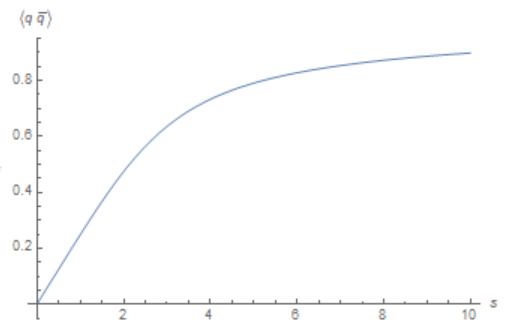
\includegraphics[width=10cm]{Capture.PNG}
    \caption{Caption}
    \label{fig:my_label}
\end{figure}
\section{On the temperature-time equality}
If we remember that in the Schrödinger picture time evolution of a statevector was given by
\be
\ket{\Psi(x,t)}=e^{-i\ham t}\ket{\psi(x,t)}
\ee
So the probability amplitude of transitioning from an initial state $\ket{\psi_i}$ to a final state $\ket{\psi_f}$ is:
\[
\mel{\psi_f}{e^{-i\ham t}}{\psi_i}
\]
If we want to know that the amplitude is for every statevector to go back to it's original state at a time $t$ we then just get:
\[
\sum_n\mel{\psi_n}{e^{-i \ham t}}{\psi_n}
\]
If we define an "imaginary time" $\tau$ as:
\[
\tau =-i t
\]
we can write
\be
\sum_n\mel{\psi_n}{e^{\tau \ham}}{\psi_n}
\ee
Now the probability for the system to be in the same state after a period of time certainly sounds like statistical mechanics. If we look at the the partition function in the Canonical Ensemble in equilibrium:
\be
Z=\Tr[e^{\beta \ham}]=\sum_n \mel{\psi_n}{e^{\beta \ham}}{\psi_n}
\ee
We see that if we equate $\beta$ with $\tau$ we get a way to go from amplitudes to the partition function. This is why we can write
\[
\tau=\beta
\]
We can extend this to the path integral version of partition function. Remember how we calculated the propagator using a path integral:
\[
K=\mel{\psi_f}{e^{-i\ham t}}{\psi_i}=\int \PD[x]e^{i\int_V\Lar \:\dd x}
\]
Now again if we set the initial state to be the final state and sum over all states we can do the substitution $\tau=\beta$ just as before. We then get that the path integral is equal to the partition function if we replace the action integral's integration variable $it\rightarrow -\tau =-\beta$:
\[
Z=\sum_n\mel{\psi_n}{e^{\beta\ham}}{\psi_n}=\sum_n\mel{\psi_n}{e^{-\tau\ham}}{\psi_n}=\int \PD[x]e^{-\int_{V^4}\Lar \:\dd x},\hspace*{1.5cm}V^4=L\times L \times L \times \beta
\]
\section{Wigner Surmise}
\be
Z=\int e^{-\Tr \ham^2}\:\dd \ham
\ee
\be
\ham =
\begin{pmatrix}
h_{11} & h_{12}\\
h_{21} & h_{22}
\end{pmatrix}
\ee
where $h_{12}=h_{21}$
\be
\ham=O\begin{pmatrix}
\lambda_1 & 0\\
0 & \lambda_2
\end{pmatrix}O^T
\ee
\be
O=\begin{pmatrix}
\cos \theta & \sin\theta\\
-\sin\theta & \cos \theta
\end{pmatrix}
\ee
\be
\dd\ham=\dd h_{11}\:\dd h_{12}\:\dd h_{22}=|J|\:\dd\lambda_1\:\dd \lambda_2\:\dd \theta
\ee
\be
J=\lp| \begin{pmatrix}\partial_{\lambda_1}h_{11} & \partial_{\lambda_2}h_{11} & \partial_{\lambda_3}h_{11} \\
\partial_{\lambda_1}h_{12} & \partial_{\lambda_2}h_{12} & \partial_{\lambda_3}h_{12}
\\
\partial_{\lambda_1}h_{22} & \partial_{\lambda_2}h_{22} & \partial_{\lambda_3}h_{22} 

\end{pmatrix} \rp|
\ee
\[
J=\lp| \begin{pmatrix}
\cos^2\theta & \sin^2\theta & (\lambda_2-\lambda_1)\sin2\theta \\
-\cos\theta\sin\theta& \cos\theta \sin\theta & (\lambda_2-\lambda_1)\cos2\theta
\\
 \sin^2\theta &\cos^2\theta & (\lambda_1-\lambda_2)\sin2\theta
\end{pmatrix} \rp|
\]
\be
|J|=|\lambda_1-\lambda_2|
\ee
\section{Winding number and shape of box}
\be
\Lar=\frac{1}{4g^2}G^a_{\mu\nu}G_a^{\mu\nu}-i\omega\theta-i\bar q \D q+\bar q_R \mathcal{M} q_L + \bar q_L \mathcal{M} q_R 
\ee
where
\be
\omega(x)=\frac{1}{32\pi}G^a_{\mu\nu}G_a^{\mu\nu},\hspace*{1.5cm}\D=\gamma^\mu\lp( \partial_\mu+iG_\mu \rp)
\ee
\be
Z=\Tr[e^{-H\beta}]=\int e^{\int_V\Lar\:\dd x }\:\PD[x]
\ee
\begin{figure}[hb]
    \centering
    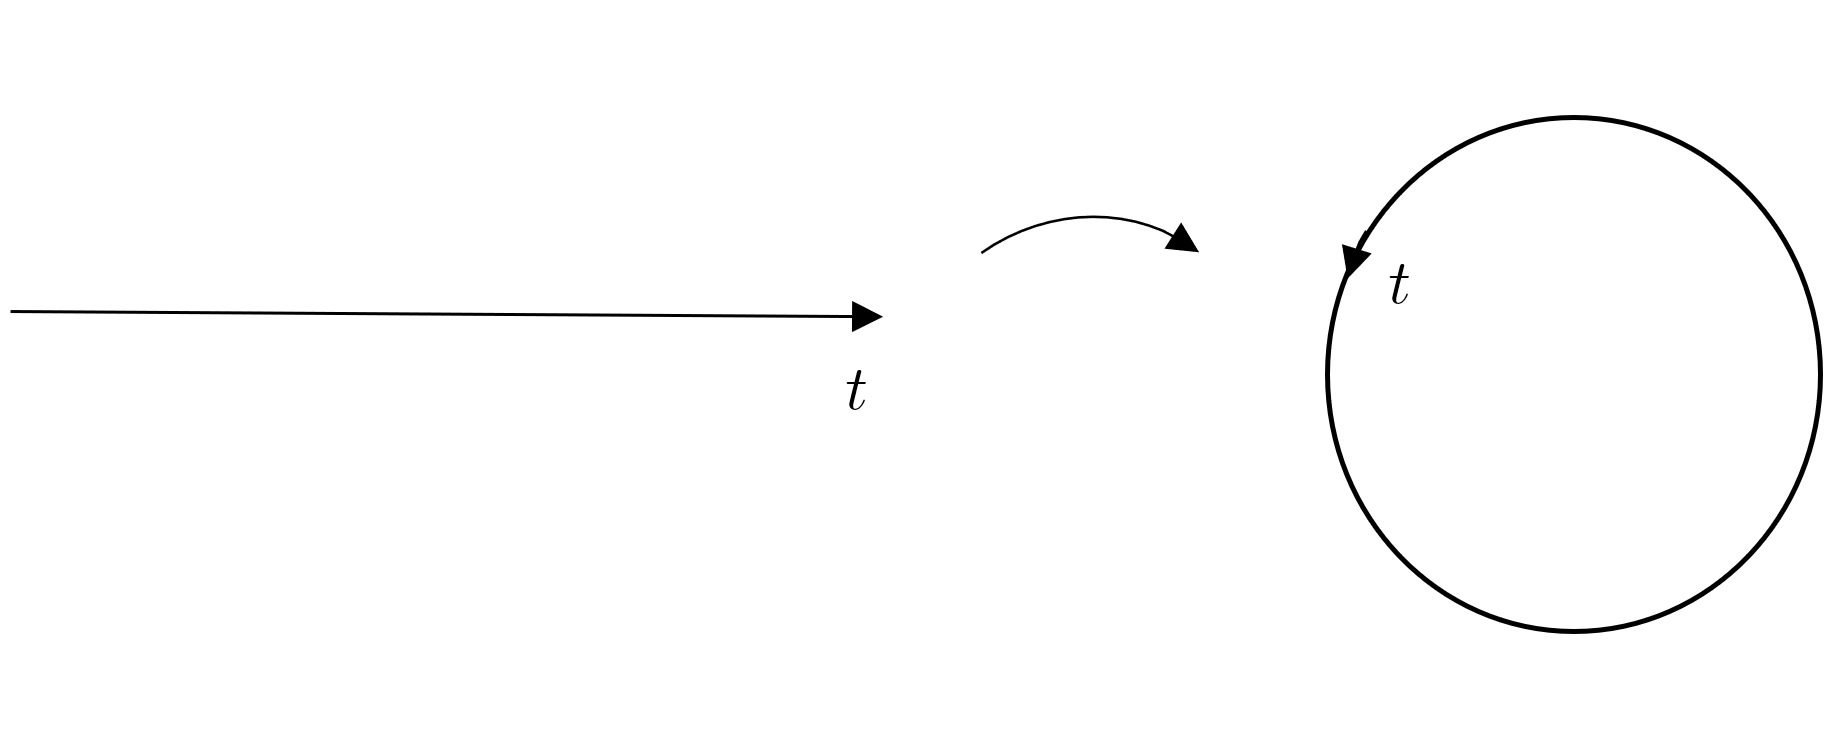
\includegraphics[width=10cm]{time.PNG}
    \caption{Curled up time dimension}
    \label{fig:my_label7}
\end{figure}
\begin{figure}[htb]
    \centering
    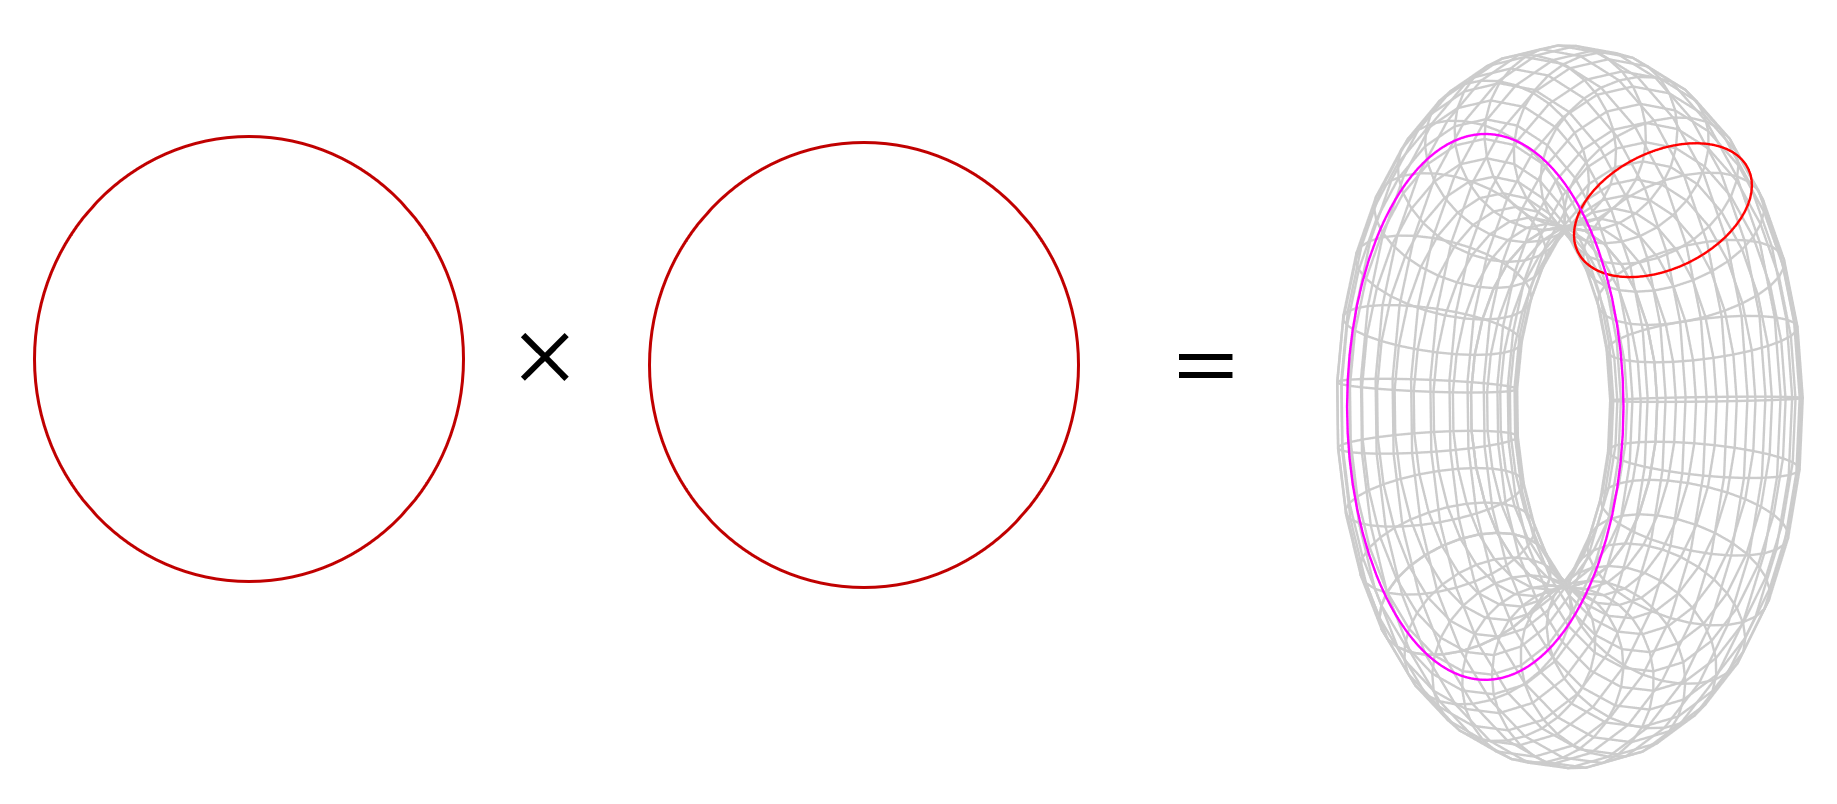
\includegraphics[width=12cm]{torus.PNG}
    \caption{Topology of torus}
    \label{fig:my_label}
\end{figure}
\be
T^n=(S^1)^{\ot n}
\ee
\begin{align}
    G_\mu (x)&=G_\mu(x+L)\\
    q(x)&=-q(x+L)
\end{align}
\be
G_\mu(x+a)=\Omega_aG_\mu \Omega_a^\dagger-i\Omega_a\partial_\mu\Omega_a^\dagger
\ee
\[
\Omega_a(x)\in SU(n_c)
\]

\subsection{Winding number and vacuum angle: Extending group integrals}
The partition function can be decomposed in its winding number components:

\be
Z=\sum_{v=-\infty}^{\infty}e^{i\theta v}Z_v
\ee

Similarily $Z_v$ can be expressed as the Fourier transform of $Z$:

\be
Z_v=\frac{1}{2\pi}\int_0^{2\pi}\dd\theta e^{-i\theta v}Z
\ee

It is evident that the winding number $v$ and the vacuum angle $\theta$ are each others Fourier conjugates. Taking $U=U_0 e^{-i\frac{\theta}{N_f}}$ yields:

\be
Z_v=\frac{A}{2\pi}\int_0^{2\pi}\dd\theta e^{i\theta v}\int_{\text{SU}(N_f)}\dd\mu(U_0)e^{s\Re{\Tr{U^\dagger}}}=A\int_{\text{U}(N_f)}\dd\mu(U)\det{U}^v e^{s\Re{\Tr{U^\dagger}}}
\ee

We know that the measures of U$(1)$ and SU$(N_f)$ can be multiplied to yield the measure of U$(N_f)$, so the Fourier transform extends the group integral from SU$(N_f)$ to U$(N_f)$.
\section{Grassmann Path Integrals}
\subsection{Basics}
First let us establish what Grassman variables are. They are elements defining an algebra of anticommutating numbers:
\be
\theta_i\theta_j+\theta_j\theta_i=0
\ee
The most important feature however is that:
\be
\theta_i^2=0
\ee
Which means that for any function $f$ of a Grassmann variable $\theta$, the first order expansion is exact:
\be
f(\theta)=a+b\theta
\ee
\subsection{Grassmann integrals}
Grassmann integrals are not ordinary, and their properties are uniquely defined by
\be
\int\:\dd \theta=0,\hspace*{1cm}\int \theta \:\dd \theta=1
\ee
Since every function can be written as $f(\theta)=a+b\theta$ this means that the integral has the same proporties as the derivative:
\be
\int f(\theta)\:\dd\theta \equiv \partial_\theta f(\theta)
\ee
Now for a multivariable function the integral depends on the order of the integrands. As an example we have:
\be
\int \theta_1\theta_2 \:\dd \theta_1\:\dd \theta_2=-\int \theta_2\lp( \theta_1 \:\dd \theta_1\rp)\:\dd \theta_2=-1
\ee
We can use this to calulate the following integral (which we'l use underneath):
\be \label{eq:grassmann}
\int \lp(a-b\theta_1\theta_2\rp)\:\dd \theta_1\:\dd \theta_2=b
\ee
\subsection{The QCD partition function for fermions without a mass term}
Let us now use these Grassmann variables to calculate the partiton function for a fermion field. We have:
\be
Z_{QCD}=\int e^{-\int \bar \psi \D \psi\:\dd x}\:\PD[\psi]\:\PD[\bar\psi]
\ee
The dirac operator satisfies the following eigenvalue equation:
\be
\D d_n=\lambda_n d_n
\ee
If we expand our Fermion fields in this basis we get:
\be
\psi=\sum c_n d_n,\hspace*{1.5cm}\bar\psi=\sum \bar c_n d_n^\dagger
\ee
where $c_n$ and $\bar c_n$ are Grassmann variables. Changing the integration variable we then have to change the path integral variable:
\[
\dd\psi\:\dd\bar\psi=\dd c_n\: \dd\bar c_n
\]
\be
\PD[\psi]\PD[\bar\psi]=\prod_{n}\dd c_n\:\dd\bar c_n
\ee
If we insert this our Lagrangian we get:
\begin{align}
\bar\psi \D \psi&=\sum_m \bar c_m d_m^\dagger \D \sum_n c_n d_n\nonumber\\
&=\sum_m \bar c_m d_m^\dagger \sum_n c_n \underbrace{\D d_n}_{\lambda_n d_n}\nonumber\\
&=\sum_{m,n} \bar c_m d_m^\dagger c_n \lambda_n d_n\nonumber\\
&=\sum_{m,n}   \lambda_n \bar c_m c_n d_m^\dagger d_n
\end{align}
Now calculating the action integral over this we get a dirac-$\delta$ which gets rid of one of the sums:
\begin{align}
\int \bar\psi \D \psi \:\dd x&=\int \sum_{m,n}   \lambda_n \bar c_m c_n d_m^\dagger d_n \:\dd x \nonumber\\
&= \sum_{m,n}   \lambda_n \bar c_m c_n \underbrace{\int d_m^\dagger d_n \:\dd x}_{\delta_{nm}} \nonumber\\
&=\sum_{n}   \lambda_n \bar c_n c_n
\end{align}
Using the fact that a sum exponated can be expressed as a product of exponentials and that the first order Taylor expansion is exact for the Grassmann variables we can express this as a product of Grassmann integrals:
\begin{align}
Z&=\int e^{-\sum_{n}   \lambda_n \bar c_n c_n}\prod_{n}\dd c_n\:\dd\bar c_n\nonumber\\
&=\int\prod_n  e^{  -\lambda_n \bar c_n c_n}\prod_{n}\dd c_n\:\dd\bar c_n\nonumber\\
&= \int\prod_n  \lp(1-\lambda_n \bar c_n c_n\rp)\prod_{n}\dd c_n\:\dd\bar c_n\nonumber\\
&=\int (1-\lambda_1\bar c_1c_1)\:\dd c_1\:\dd\bar c_1\times \int (1-\lambda_2\bar c_2c_2)\:\dd c_2\:\dd\bar c_2 \times \cdots
\end{align}
Using the integral identity for Grassmann integrals (eq: \ref{eq:grassmann}) we then get
\begin{align}
Z&=\prod_n \lambda_n\nonumber\\
&=\det\D
\end{align}
\subsection{With a mass term}
Now let us look at the full QCD partition function
\be
Z_{QCD}=\int e^{-\int \bar \psi (\D+m) \psi\:\dd x+S(A_\mu)}\:\PD[\psi]\:\PD[\bar\psi]\:\PD[A_\mu]
\ee'
where we have an implied sum over flavours in the Lagrangian. (This means that the determinant in the end will be raised to $N_f$ power). The term $S(A_\mu)$ is the Yang-Mill functional which we won't go into.

We now have a few things to take into account. First let us note that since $(i\D)^2$ commutes with $\gamma_5$ the two must share common eigenstates. It can be shown that this leads to the eigenstates for $\D$ splitting up in paired Left- ($-$) and Right- ($+$) handed  eigenstates $\pm \lambda$. For the zero modes this pairing does not occur.

This means that for the determinant of the two operators $\lp(i\D+m\rp)$ we can write their determinant:
\be
\det \lp(\D+m\rp)=m^v
\prod_n\lp( \lambda_n+m \rp)\lp( -\lambda_n+m^* \rp)=m^v 
\prod_n\lambda_n^2+|m|^2
\ee
where we have $v$ mass eigenvalues from the zero modes, and the rest is a product over the non zero-modes.

Using the result obtained in the previous section we can then generalize the partition function to:
\be
Z(m)=m^{N_fv}\int\lp[\prod_n\lp(\lambda_n^2+m^2  \rp)\rp]^{N_f}e^{S(A_\mu)}\:\PD[A_\mu]
\ee
We see that that if we change the mass by a phase
\[
m\rightarrow me^{i\theta}
\]
the partition function changes accordingly
\[
Z\lp(me^{i\theta}\rp)=\lp(me^{i\theta}\rp)^v\int\prod_n\lp(\lambda_n^2+m^2  \rp)e^{S(A_\mu)}\:\PD[A_\mu]=e^{iv\theta}m^v\int\prod_n\lp(\lambda_n^2+m^2  \rp)e^{S(A_\mu)}\:\PD[A_\mu]=e^{i\theta}Z(m)
\]
We will implement this as a consistency check, since our effective partition function should obey the same feature.

\section{Calculating sanity checks for U$(2)$}

In the following we will calculate I few things and check if they behave as expected in the appropriate limits. This will be a useful tool for checking the Techni-QCD results we will later derive. 

We can check if $Z_\nu$ in the effective theory behaves as in QCD, that is:
\be
Z_v(m)\rightarrow Z_v(me^{i\theta})=Z_v(m)e^{iN_f\nu\theta}
\ee
Writing
\be
Z_v(m)=\int_{U(N_f)}\lp(\det U\rp)^v e^{\frac{f^2}{2}B_0 V\Re \Tr[MU^\dagger +M^\dagger U]}\:\dd\mu(U)
\ee
we get
\be
Z_v(me^{i\theta})=\int_{U(N_f)}\lp(\det U\rp)^v e^{\frac{f^2}{2}B_0 V\Re \Tr[Me^{i\theta}U^\dagger +M^\dagger e^{-i\theta}U]}\:\dd\mu(U)
\ee
Changing variables 
\be
U\rightarrow V=e^{-i\theta}U
\ee
we get:
\begin{align}
Z_v(me^{i\theta})&=\int_{V(N_f)}\lp(\det Ve^{i\theta}\rp)^v e^{\frac{f^2}{2}B_0 V\Re \Tr[MV^\dagger +M^\dagger V]}\:\dd\mu(V) \\
&=e^{iN_f\nu\theta}\int_{V(N_f)}\lp(\det V\rp)^v e^{\frac{f^2}{2}B_0 V\Re \Tr[MV^\dagger +M^\dagger V]}\:\dd\mu(V)\\
&=Z_v(m)e^{iN_f\nu\theta}
\end{align}
There is no change in the measure since we are integrating over all of U$(N_f)$ anyway. This can be seen by the fact that the absolute value of the appropriate Jacobian is 1. 
\\
\\
A good sanity check is also to verify that the partition function and topological susceptibility lives in $\mathbb{R}_+$. In addition, the topological susceptibility should also go to zero as the mass does. For U$(2)$ in QCD we can straightforwardly calculate the topological susceptibility. Generally we have:
\be
\expval{\nu^2}=\sum_\nu \nu^2\frac{Z_\nu}{Z}
\ee
But writing:
\be
Z(\theta)=\sum_\nu e^{i\theta\nu}Z_\nu
\ee
And differentiating twice:
\be
\partial_{\theta}^2 Z(\theta)=-\sum_\nu \nu^2e^{i\theta\nu}{Z_\nu}
\ee
So evidently the expression for the topological susceptibility is simply:
\be
\expval{\nu^2}=-\frac{\partial_{\theta}^2 Z(\theta=0)}{Z(\theta=0)}
\ee
In the case for U$(2)$:
\be
Z(\theta)=\frac{I_1(2s\cos\theta)}{s\cos\theta} \longrightarrow \partial_\theta^2Z(\theta=0)=-2I_2(2s)\longrightarrow \expval{\nu^2}=\frac{2sI_2(2s)}{I_1(2s)}
\ee
Interestingly, the plot of $\expval{\nu^2}$ for U$(1)$ is linear in $s$, $\expval{\nu}=s$ and in the U$(2)$ case it looks quadratic near the origin and linear away from the origin. This invites the conjecture that the topological susceptibility will grow as $s^{N_f}$ near zero and linear away from it. This is probably not difficult to either verify or disprove. 
\\
\\
A different test is to plot the condensate and check if it behaves expectedly in the appropriate limit. So far we see that if the volume is kept finite and the mass goes to zero then the condensate must also go to zero. 
\\
\\
Plotting $\frac{Z_\nu}{Z}$ for constant $m$ and $\theta=0$ for different $\nu$ is also a way of checking if our theory behaves as expected.

\section{Preliminary understanding of Golterman and Shamir}

In their paper they investigate a techni-QCD theory in which they have both a chiral symmetry, confinement and a walking of the coupling. The walking of the coupling is embodied in the beta function:
\be
\beta(g)=\mu\frac{\partial g}{\partial \mu}
\ee
Where $g$ is the coupling and $\mu$ is the energy. Therefore the beta function tells us how fast the coupling changes as the energy changes and we thus achieve the walking regime when beta approaches zero. The walking endows the theory with an additional symmetry besides the chiral symmetry and that is a scaling symmetry. In the framework of (pseudo) Nambu-Goldstone bosons it seems that this scale invariance gives rise to a new scalar meson. 

In order to smoothly control the beta function they take the same large $N_c$ limit where $n_f=\frac{N_f}{N_c}$ is kept fixed and finite. This is called the Veneziano limit. The regime, the paper investigates, are then values $n_f<n_f^*$ where $n_f^*$ is the lowest value for which $\beta=0$. The paper argues that in order to control the walking smoothly they need to take both the Veneziano limit and the limit $n_f\longrightarrow n_f^*$. \edit{But I have one note:} It seems that the different regimes actually allow for four different limits: The small mass limit, the large $N_c$ limit ('t Hooft limit), the Veneziano limit (both $N_f, N_c \longrightarrow \infty$) and then finally the walking limit, $n_f \longrightarrow n_f^*$ (which is dependent on the Veneziano limit). The interesting aspect is the following: What is the difference between taking the 't Hooft limit only and not the Veneziano limit? It is difficult to read how everything behaves in the different limits.

\edit{Okay, so I thought I understood this, but I don't:} To understand the connection between a walking theory and scale invariance we look at the scaling of the different terms that is associated with energy and coupling:

\be
A_\mu(x)\longrightarrow \lambda A_\mu(\lambda x) \ ; \ \chi(x)\longrightarrow\lambda \chi(\lambda x)
\ee

So the scaling demands a change in the magnitude of both $A_\mu$ and $\chi$. We interpret the new magnitude of the gauge field as an increase in the coupling and the new mass term to be an increase in the energy. Thus, if changing 
\subsection{The U$_A(1)$ anomaly}
So far we've been working with SU-groups which have been extended by introducing the axion field and thus the vacuum angle. This enables us to perform an additional (Fourier) integration which expands to U-groups. In the large $N_c$ limit, however, the U$(1)_A$ anomaly, which the axion field compensates for, is vanishing. Therefore the relevant groups is naturally extended to U-groups and it seems superfluous to include the axion field and consequently \edit{the winding number}.

The breakdown from the formation of the chiral condensate goes as
\[
\SU_R(N_f)\ot\SU_L(N_f)\ot\U_V(1)\rightarrow\U_V(N_f)
\]
resulting in $\lp[(N_f^2-1)+(N_f^2-1)+1^2\rp]-N_f^2=17-9=8$ broken generators and therefore 8 Nambu-Goldstone bosons.
\end{document}

